\documentclass[journal, a4paper]{IEEEtran}
\usepackage{graphicx}  
\usepackage{subfigure}
\usepackage{url} 
\usepackage{amsmath}    
\usepackage{float}
\floatstyle{ruled}
\restylefloat{figure}  
\restylefloat{table}    
\usepackage{hyperref}
\usepackage{tabularx}
\usepackage{physics}

\begin{document}

\title{Understanding Customer Loyalty \\ in the Brazilian Economy}
\author{Darshan Patel}
\markboth{Fordham University Gabelli School of Business}{Machine Learning in Statistics}
\maketitle

\begin{abstract}
The purpose of this study is to examine shopping behaviors of Brazilian card owners. The company Elo wants to offer personalized promotions to card holders based on their purchases. Given a loyalty score for each card holder, it is the goal of the modeler to find the best explanations for it. After creating a number of regression models, it was found that the gradient boosting tree model, \texttt{XGBoost}, provided the best predictions for the loyalty scores. This model also found some important features that help determine loyalty score, such as the date of the earliest purchase date, number of transactions made and the maximum normalized purchase amount. Further feature engineering and modeling techniques can be applied to make the original features given more useful for predicting loyalty score. 

\end{abstract}

\section{Introduction}
In Brazil, Elo is one of the biggest debit and credit card providers for domestic use. It is formed by a partnership of three banks in Brazil: Banco de Brasil, Bradesco and CAIXA. Til now, Elo has issued more than $50$ million cards (credit, debit or prepaid) for use in Brazil. Elo provides an excellent payment method, where shoppers can pay off their credit card bill in installments, which allows holders to worry less about their money and think more about what they really enjoy. In fact, even Cielo, one of the largest merchant groups in Brazil, has given permission to shop owners to accept Elo in their online stores. Not just in Brazil, but all over the world, Cielo allows the payment brand Elo to be used anywhere online. 

In February 2019, Elo launched an initiation on \texttt{Kaggle} to help them boost promotional activity. The company has partnered with various merchants in Brazil to launch ads and discounts to card holders. But this is not simple to do so; an effective campaign cannot highlight nice deals for any local restaurant to just everyone. Imagine that it is late night, you are in an unfamiliar town and you are hungry. What you crave at the moment is your favorite, felijoada (black bean and pork stew) but when you check for recommendations by your best friend, Elo, all you see is offers for cheap eats at a local McDonald's. This campaign would work better if promotions can be targeted based on what consumers purchased in the past. This is the task that Elo has issued to data scientists on Kaggle. 

Elo has given various sorts of information about customers transactions and merchants for modeling use. It has also computed a loyalty score for each customer card holder. The goal of this capstone project is to find out how to explain the loyalty score. Elo has given data on three months worth of historical transactions customers have made. Along with this transaction data, there is two months' worth of data for transactions made at merchants that were not mentioned in the historical transactions data. In addition, information on merchants is also provided to see how merchants are performing. Lastly, Elo has given three features directly that can be used to understand the loyalty score, along with each cardholders' date of first month of activity. 

In this project, various steps will be taken to assemble the data together and create models. But before doing so, it is imperative to look at the data as it is to uncover insights about customers. In addition, since the datasets provided by Elo is moderately large, up to $3$ GB for the historical transactions alone, AWS instances will be utilized for the entire duration of this project. 

\section{Exploratory Data Analysis}
\subsection{Training and Testing Data}
The training and test data is first looked at. The training data is composed of $201,917$ unique card holders and $6$ variables: first active month, card ID, feature $1$, feature $2$, feature $3$ and the loyalty score. The testing data is composed of $123,623$ unique card holders and $5$ variables, all of which are the same as before with the exclusion of loyalty score. The first pieces of information that is looked at are the three feature values per card holder and their respective loyalty score. \begin{figure}[h!] 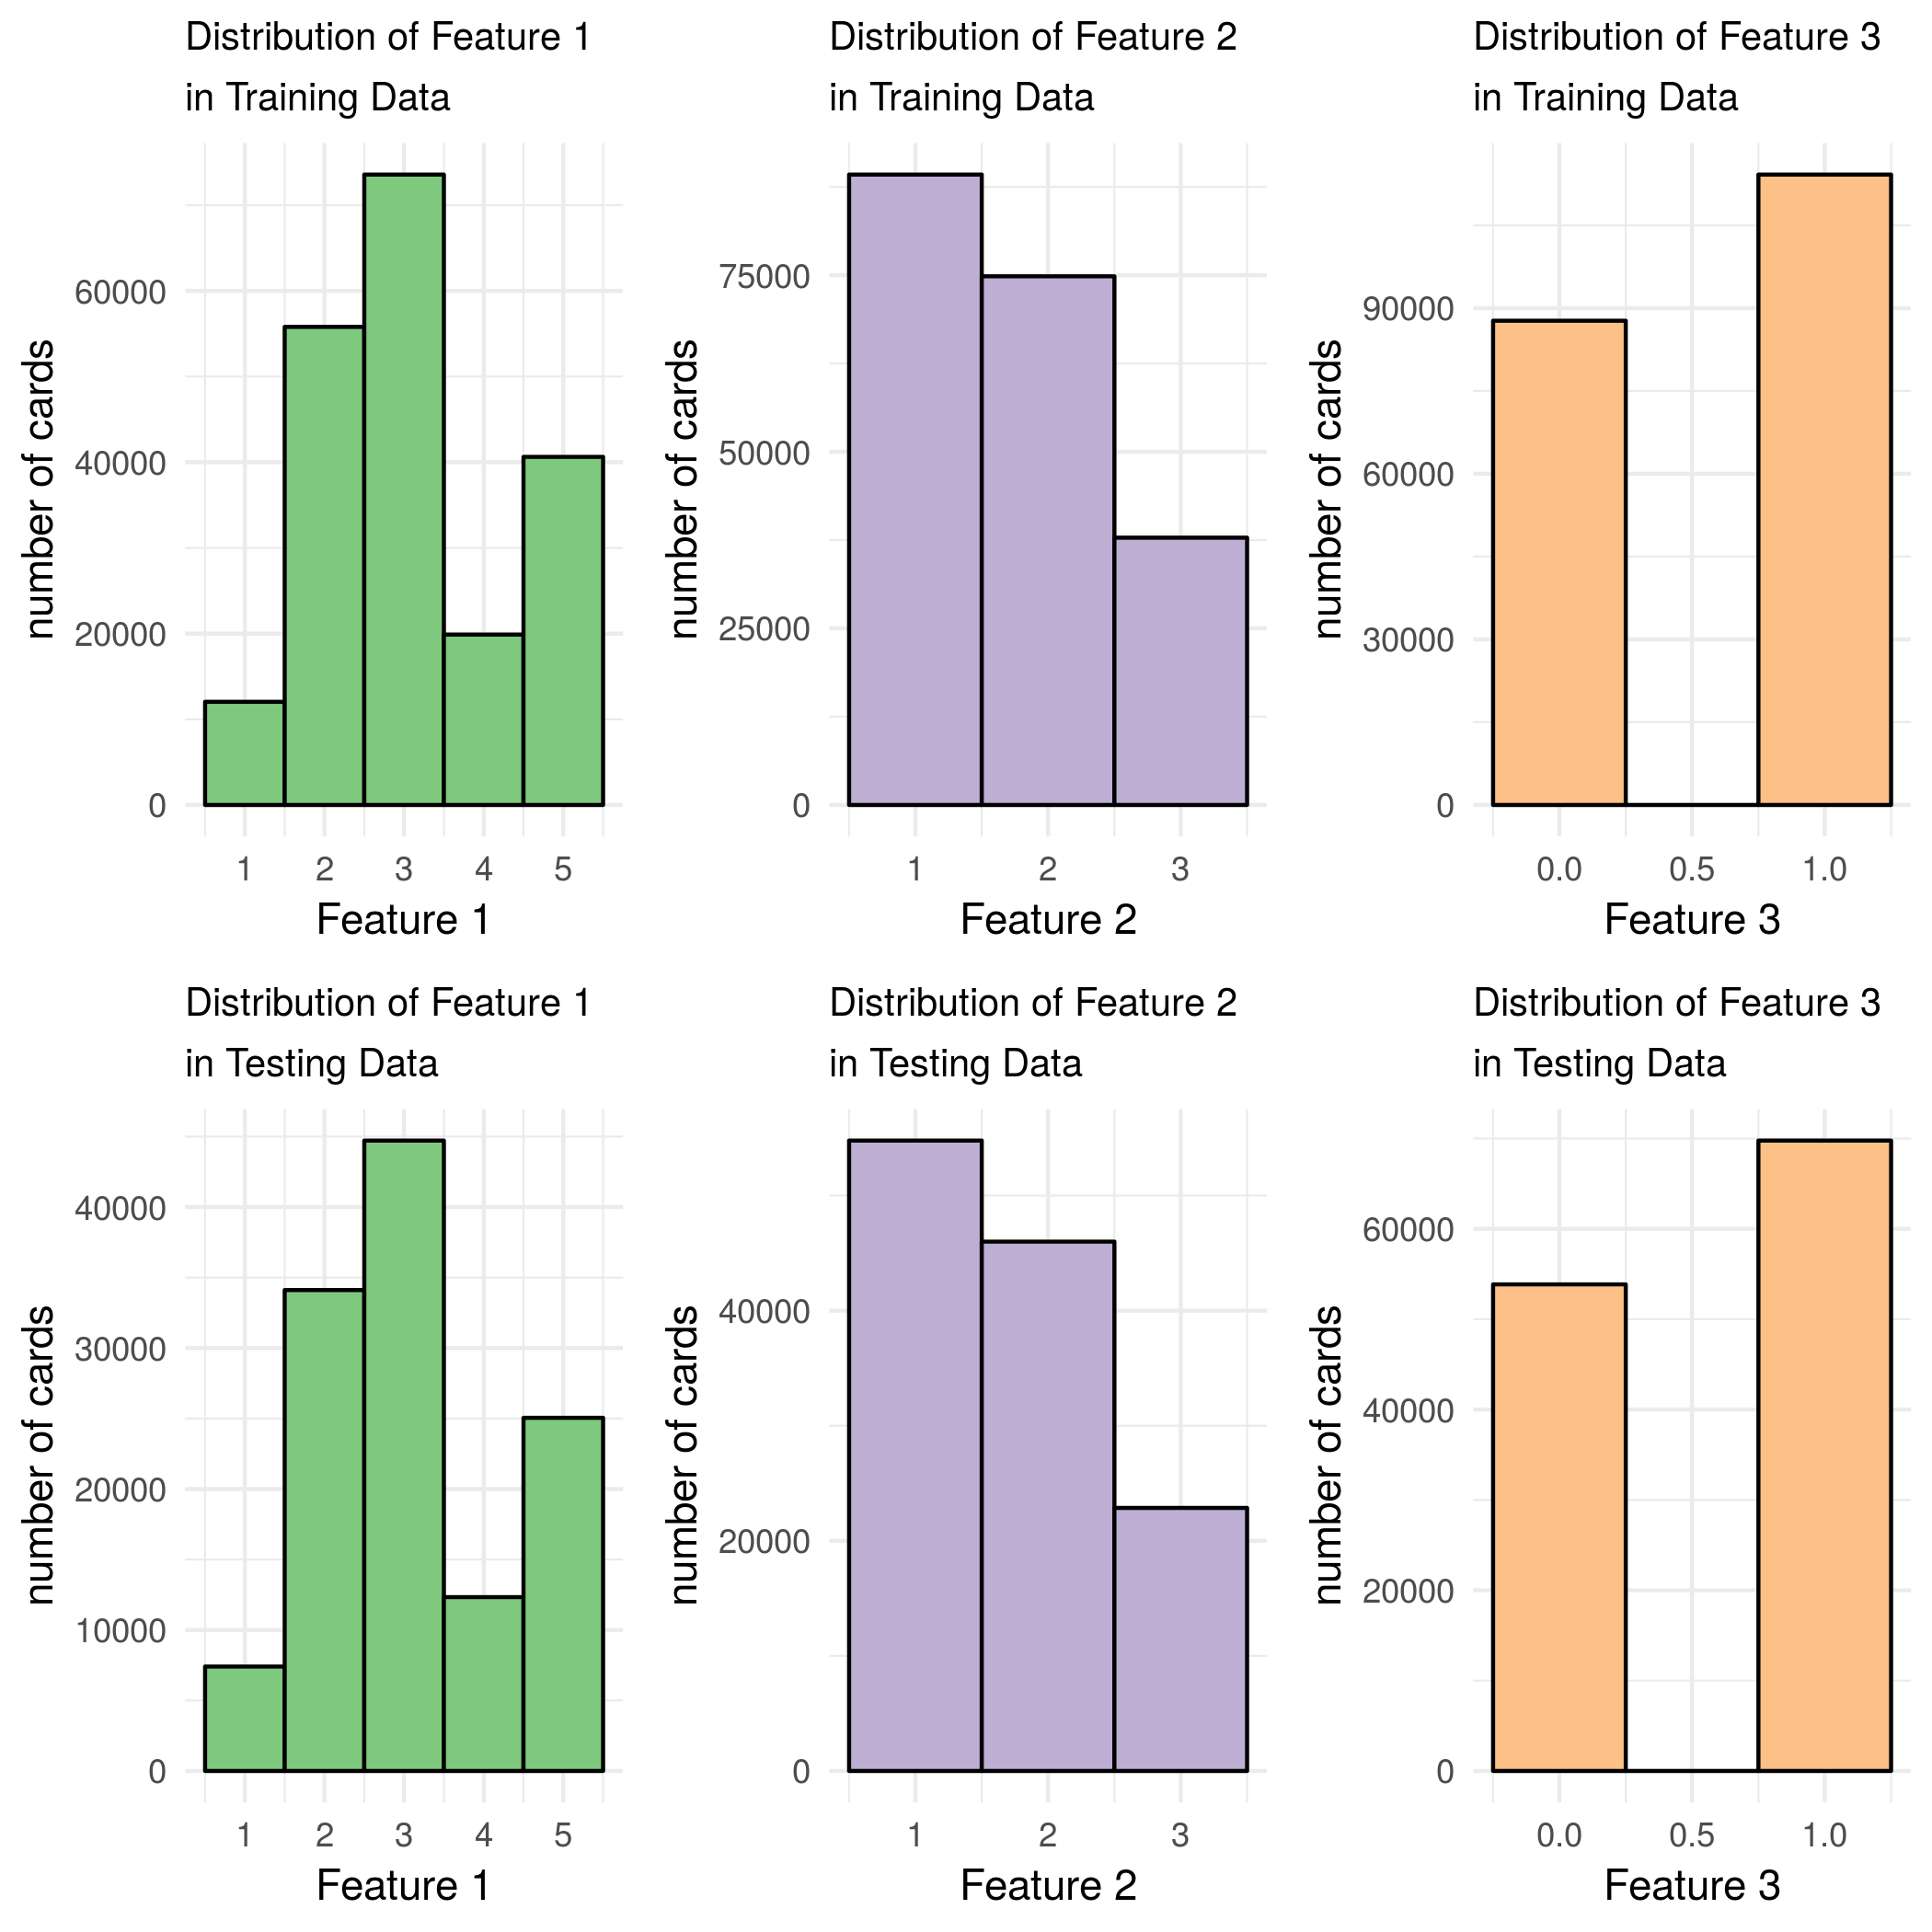
\includegraphics[scale = 0.5]{features} \caption{Distribution of features in training and testing data.} \end{figure}A number of takeaways are made about the cardholders. As seen in Fig. 1 above, it is apparent that each of the features are not identically distributed. Feature $1$ is normally distributed but skewed to the right, for both the training and testing data. Feature $2$ is skewed to the right whereas feature $3$ is skewed to the left. There is no significant difference between them in the training and testing data. Next the target score is looked at. Note that only the training data has target scores given by Kaggle.  \begin{figure}[h!] 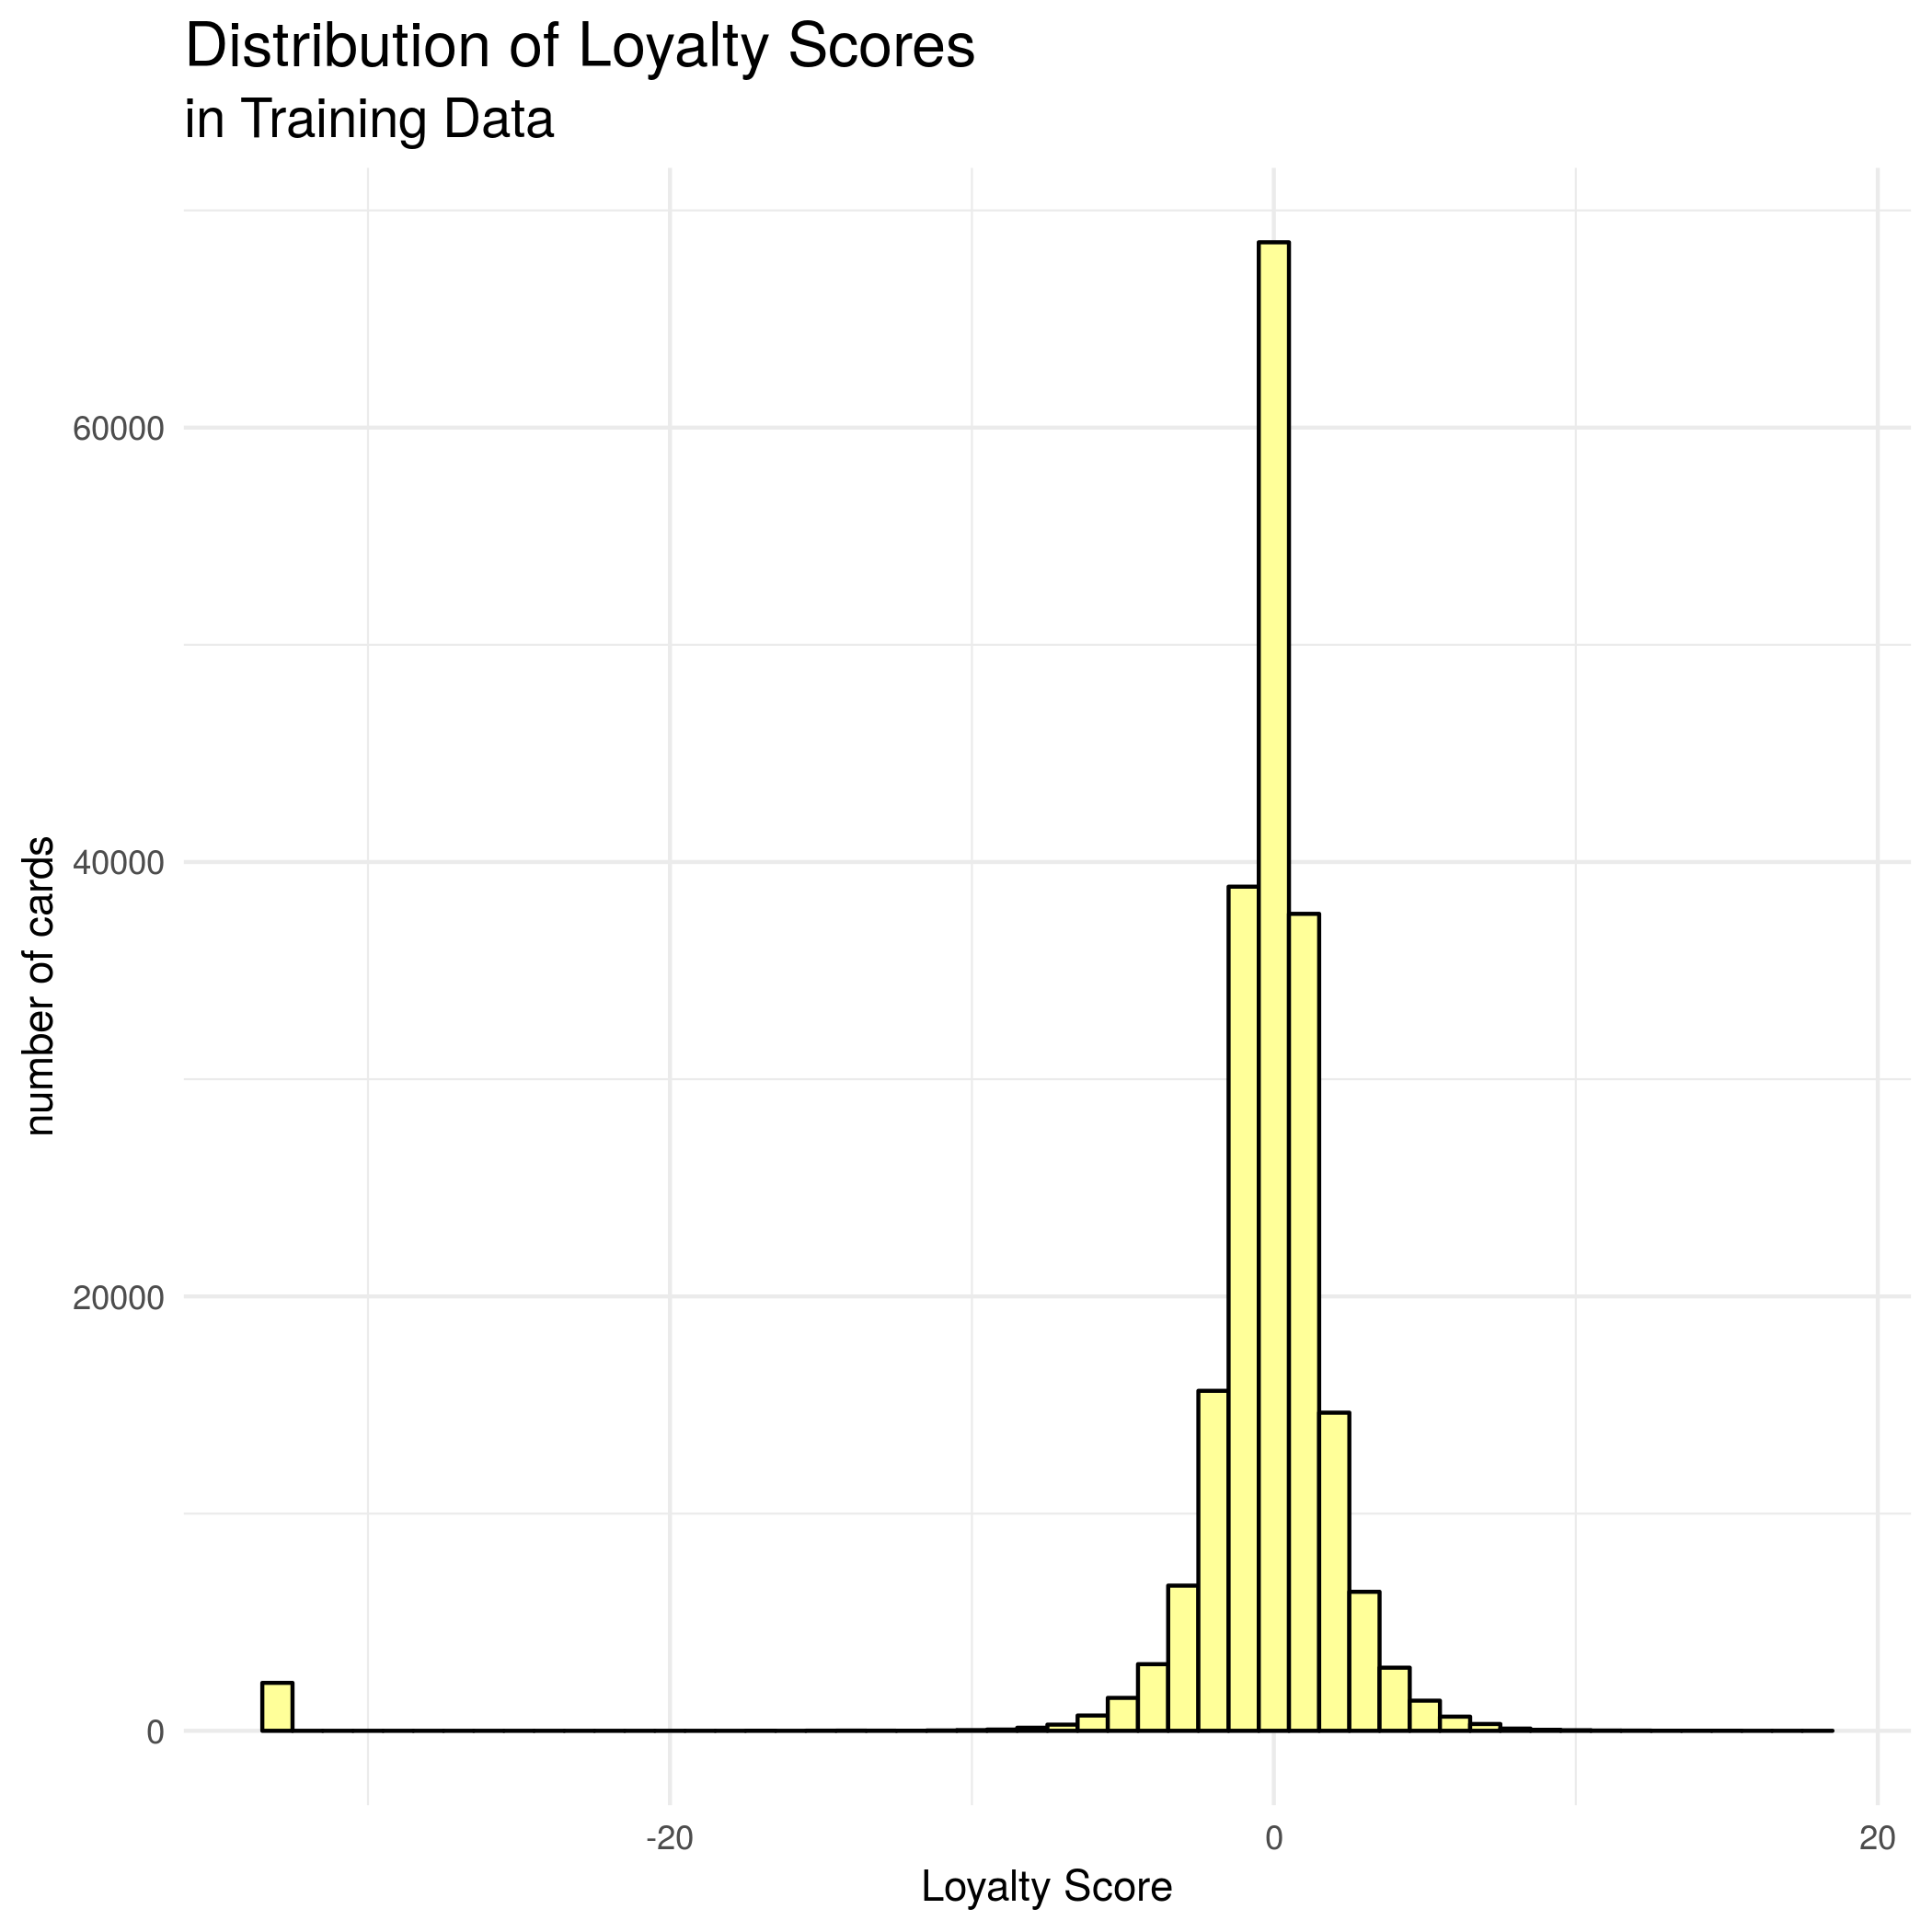
\includegraphics[scale = 0.4]{target} \caption{Distribution of target score in training data.} \end{figure}
 \begin{figure}[b] 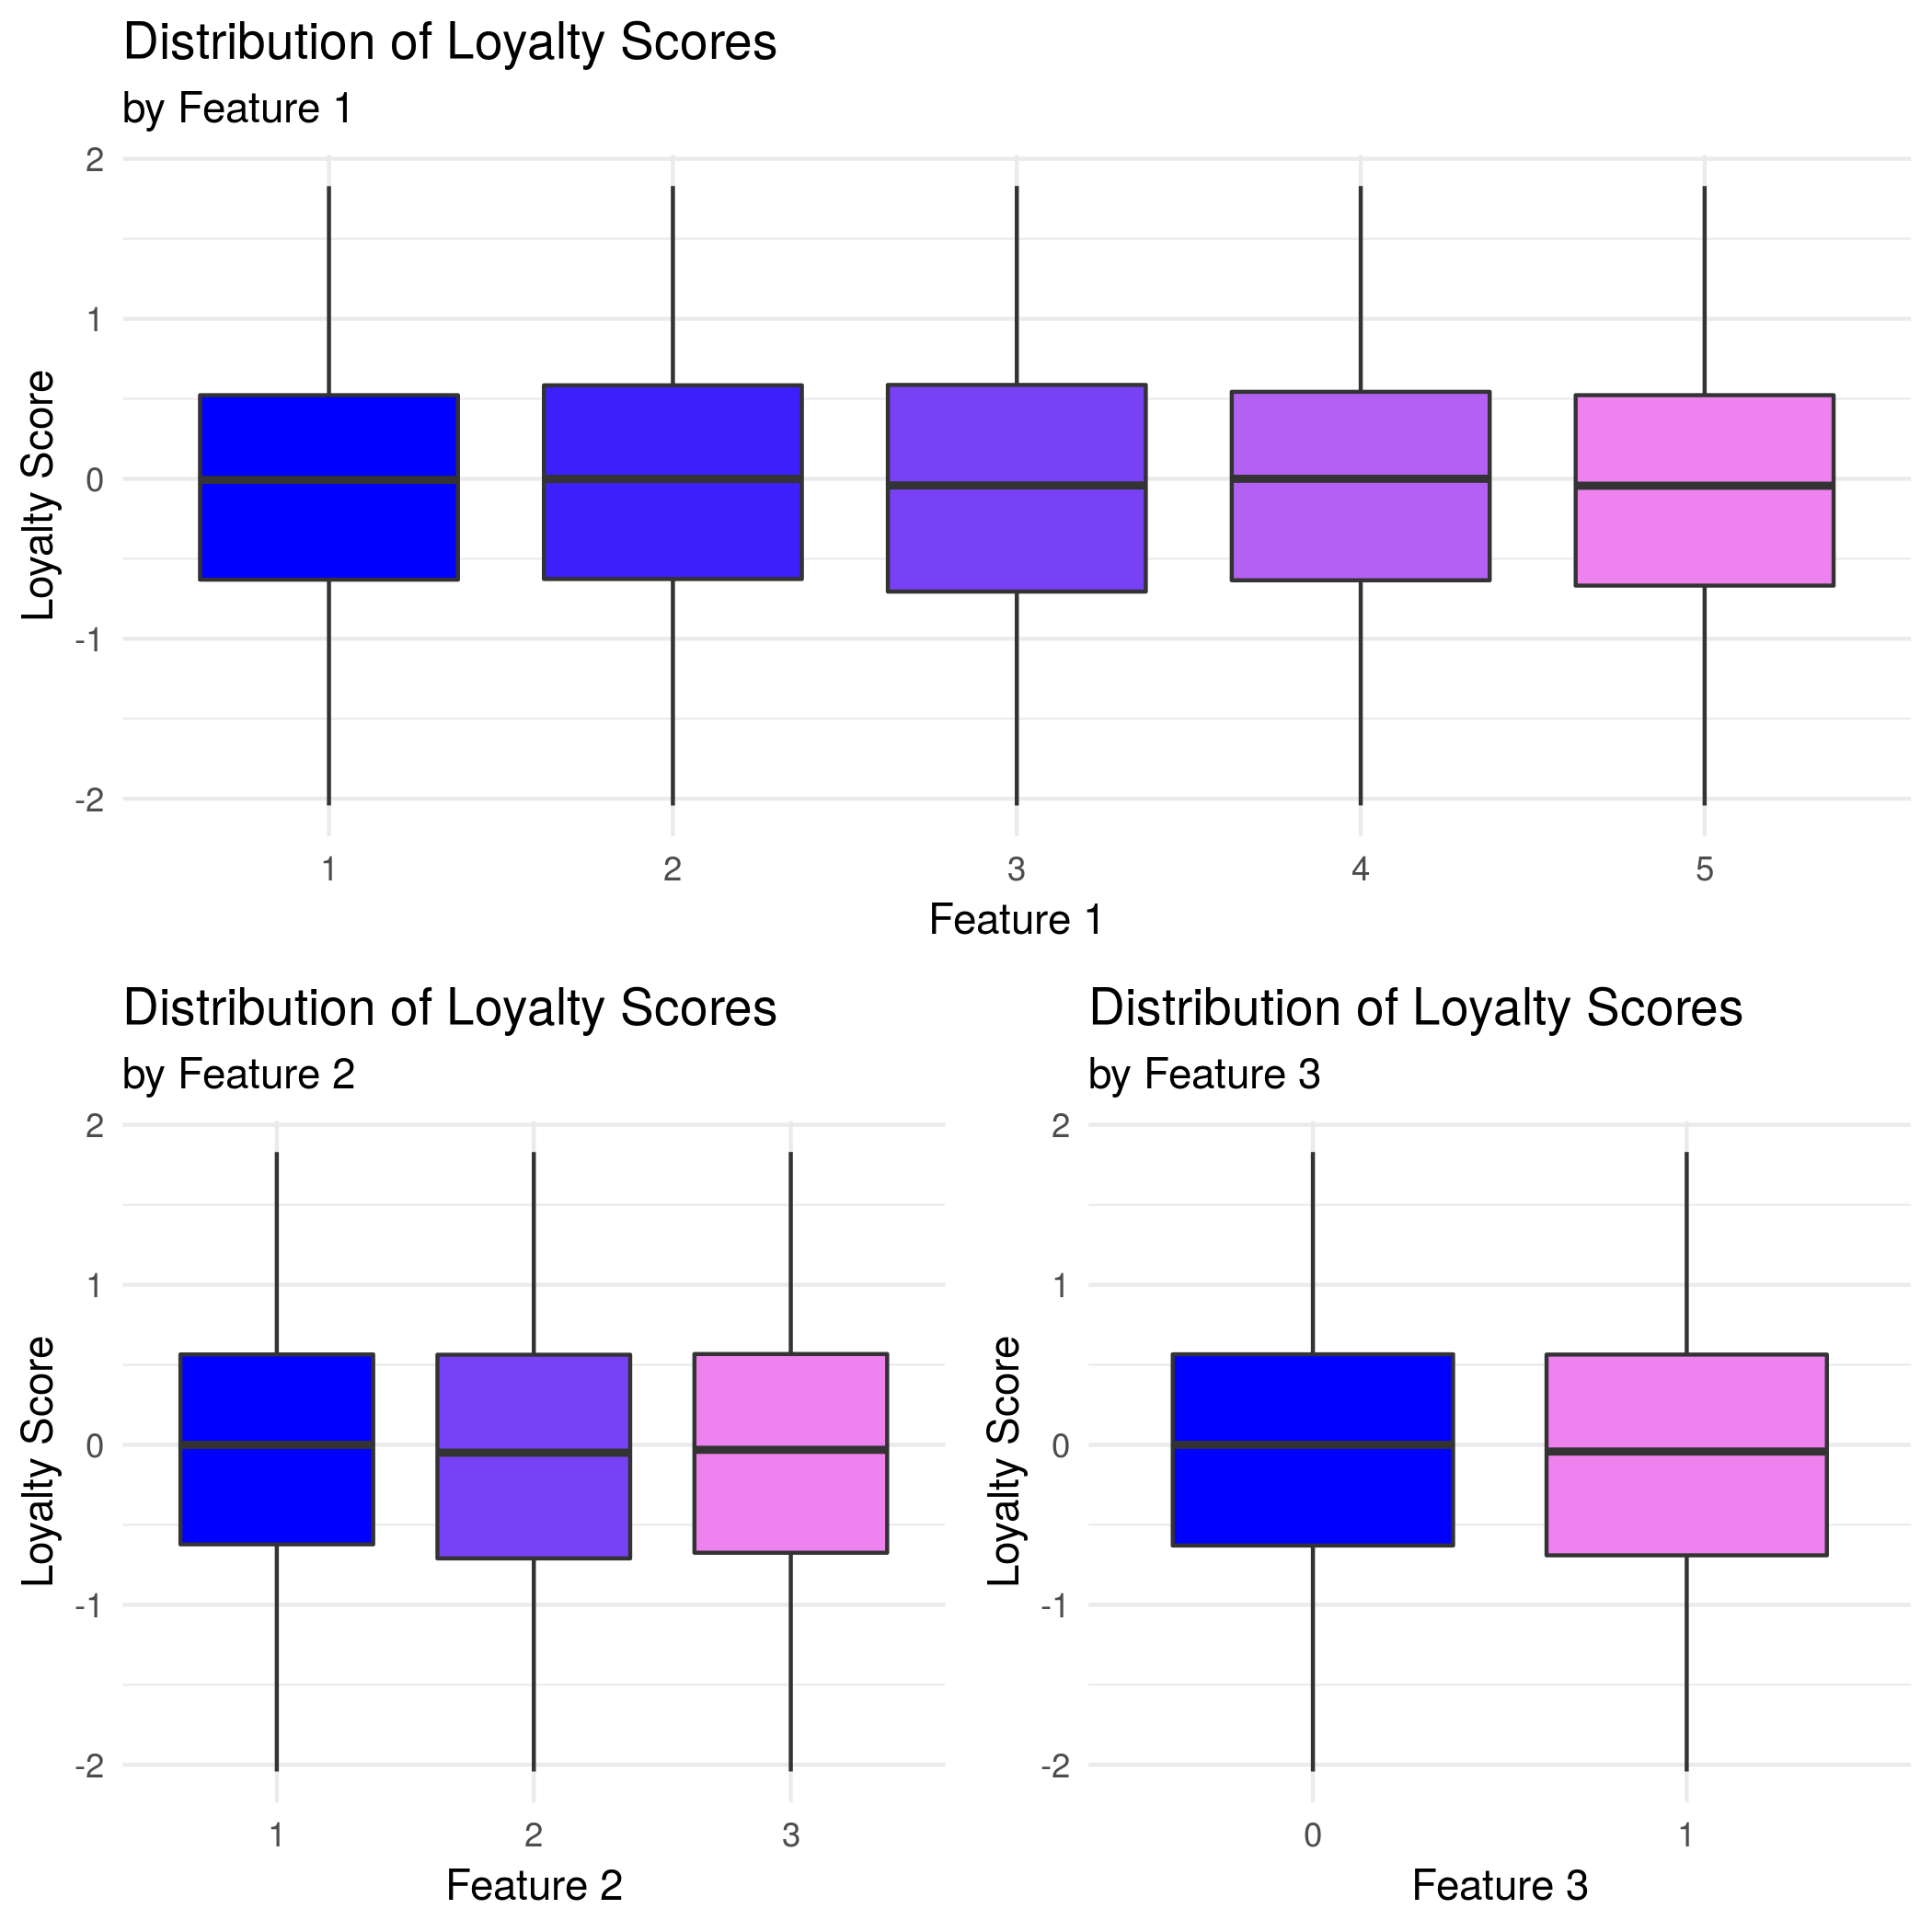
\includegraphics[scale = 0.4]{target_feat} \caption{Distribution of loyalty scores by feature value.} \end{figure}
 \begin{figure}[h!] 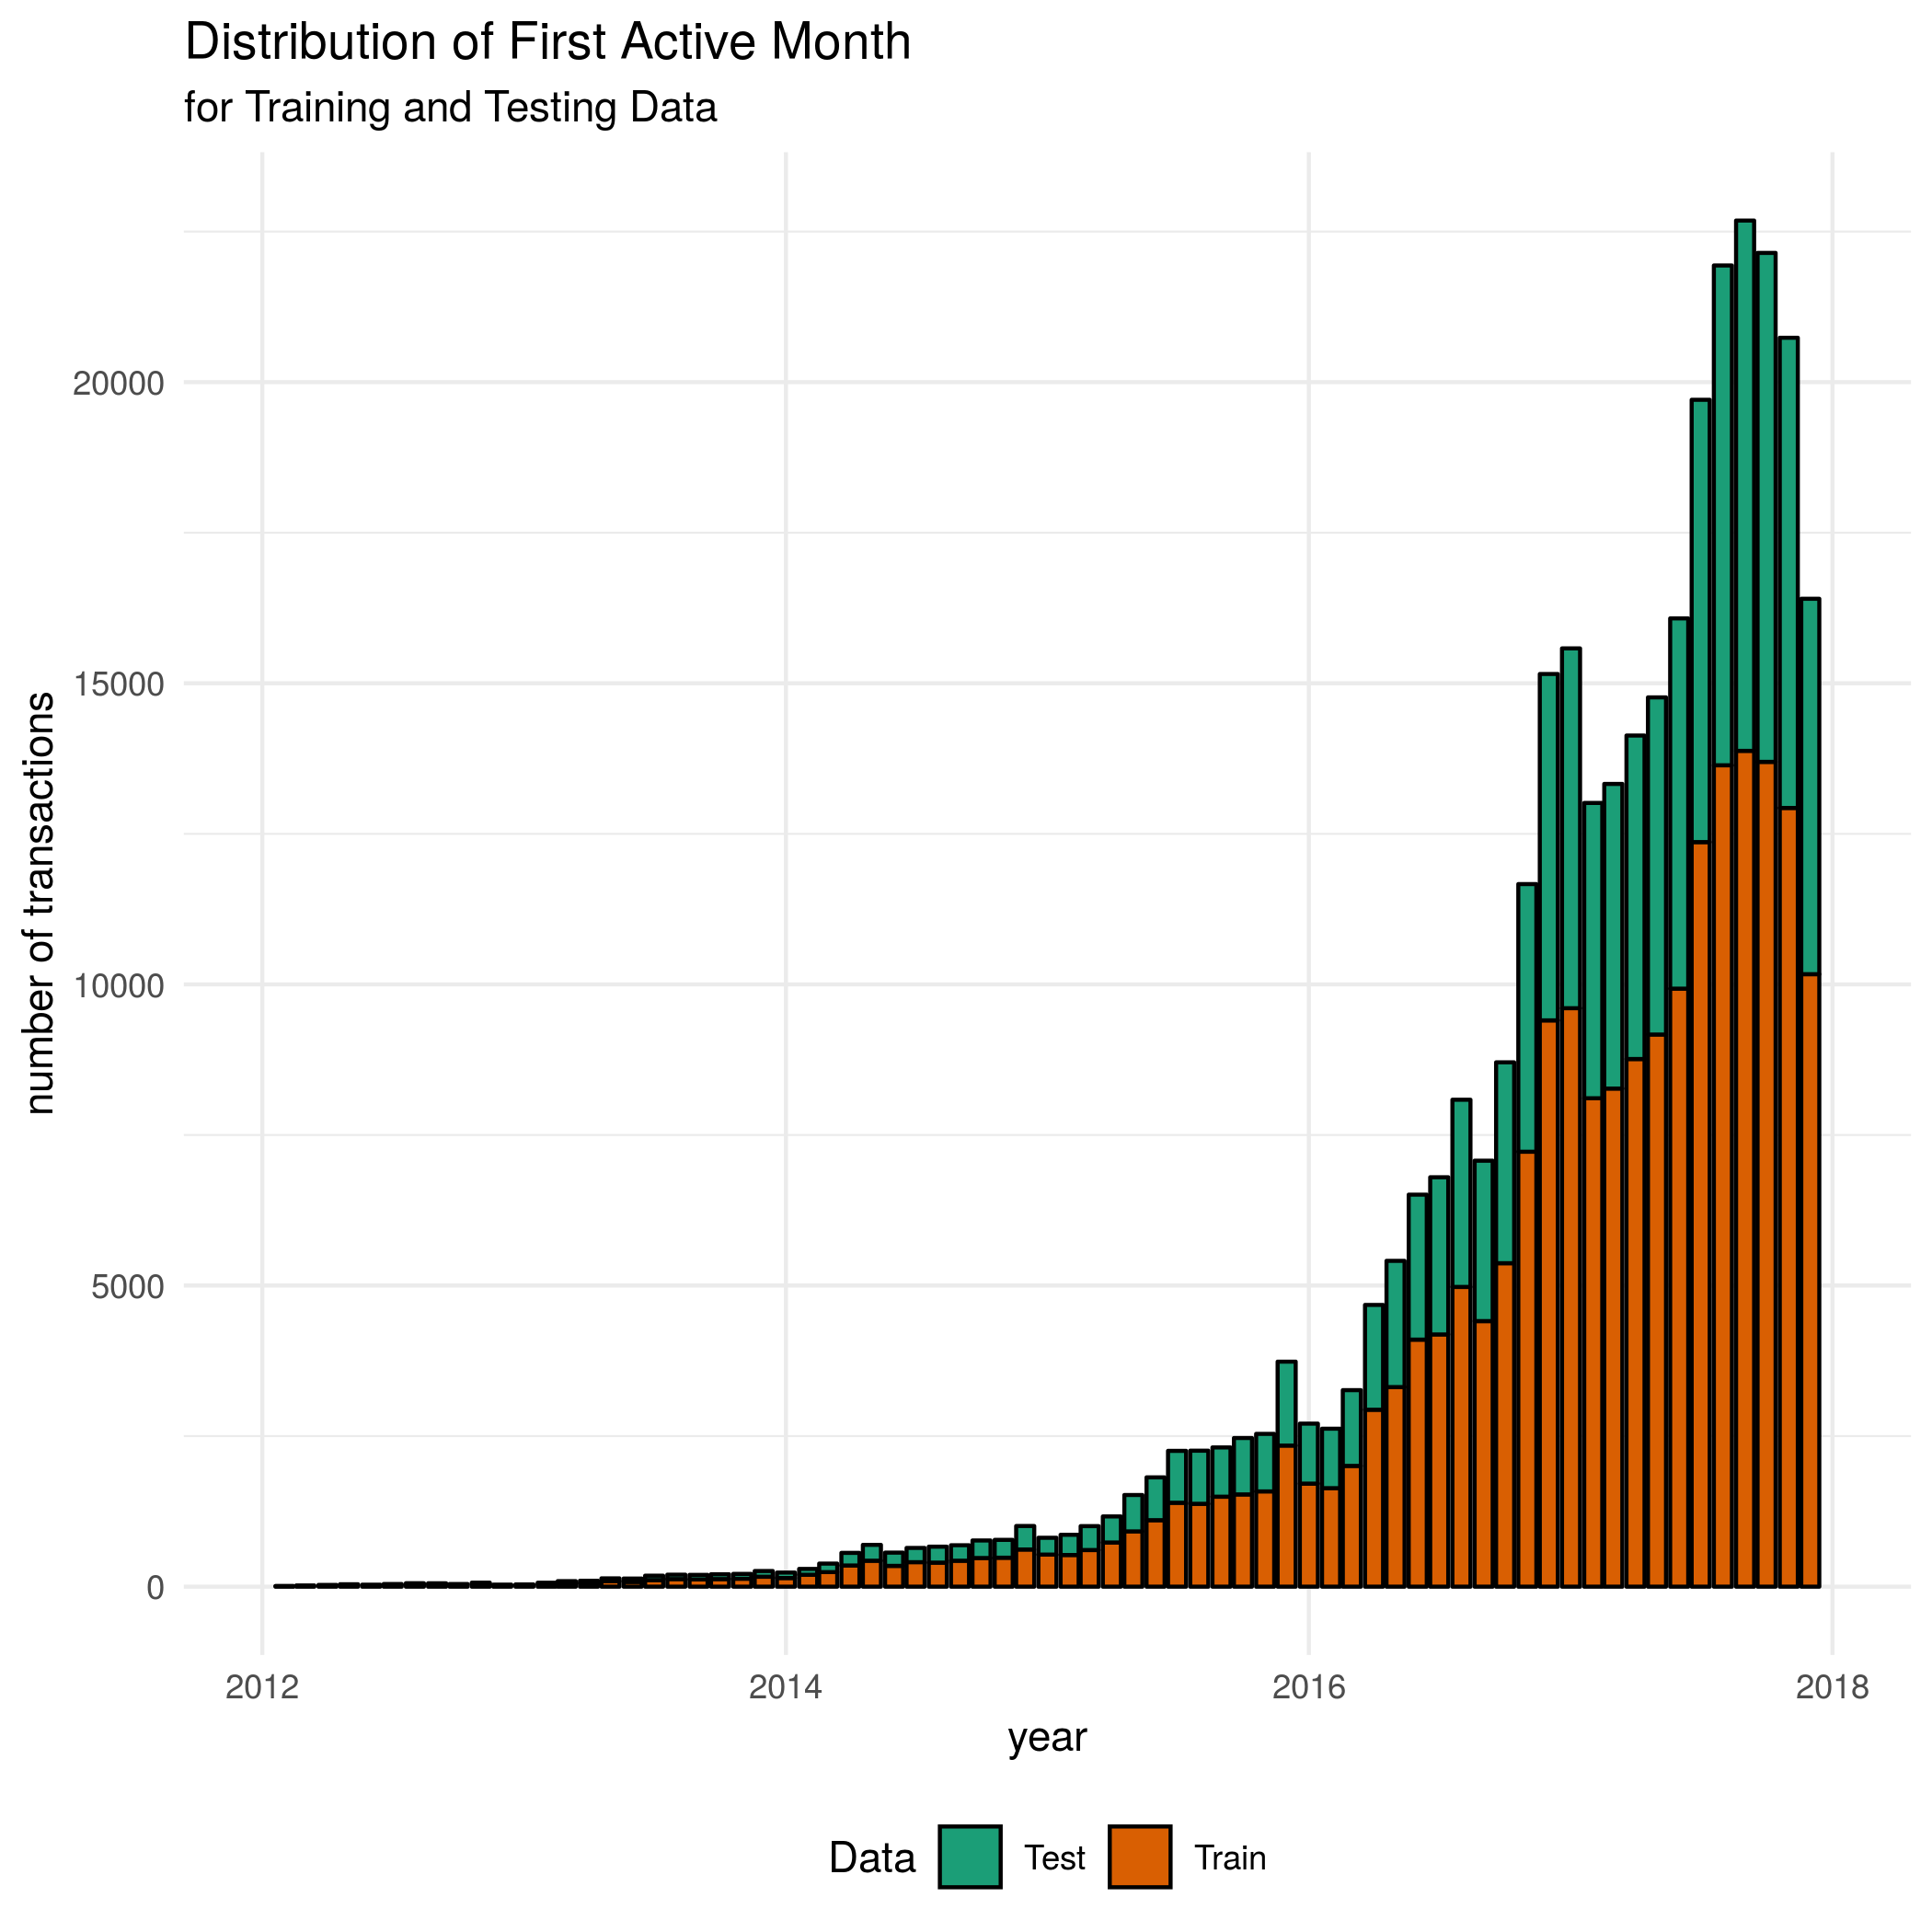
\includegraphics[scale = 0.4]{fam_plot} \caption{Distribution of transactions by first active month.} \end{figure}
The loyalty score is distributed normally as seen in Fig. 2. This suggests that Elo normalized the scores to reduce the variance in the scores amongst individuals. However, there are a small number of card holders that have a very low normalized loyalty score. A helpful thing to do now would be to examine how the target scores are distributed by the features in the training data, as shown in Fig. 3. For ease of visual interpretations, outliers (the really low loyalty scores) were removed from the box plots so that the quantiles could be looked at more closely. It is found that there is not a huge difference in loyalty score distributions amongst different values in all three features. A conclusion that can be made from this is that a typical run of the mill linear regression algorithm will not greatly explain the loyalty score, since none of the features show any distinctive distribution with loyalty scores. 

Apart from the features and loyalty scores in the training and testing data, Elo has also provided the first active month for each cardholder. It is clear that as time progresses, the number of card holders who are using Elo is growing exponentially, as shown in Fig. 4. In addition, the testing data's first month of activity is mostly after $2016$. There appears to be little to no testing data information for prior to $2014$. 

\subsection{Transactions}
Transactional data is broken into two categories: historical transactions and new transactions. The historical transactions dataset has $29,112,361$ records of transactions from a span of $3$ months. It has $14$ variables giving information about customer transactions such as: authorization flag (whether the transaction was approved), the purchase date, the month lag to the reference date, card ID, merchant identifier, merchant category identifier, merchant category group identifier, normalized purchase amount, number of installments, city and state identifiers and three anonymized categories. In the new transactions dataset, there is $2$ months worth of transactions for merchants not mentioned in the other file. It has $1,963,031$ transactions and $14$ variables. 

There are several variables that will be looked at, each with respect to type of transaction. First, the distribution of the three anonymized categories is looked at. 
 \begin{figure}[t] 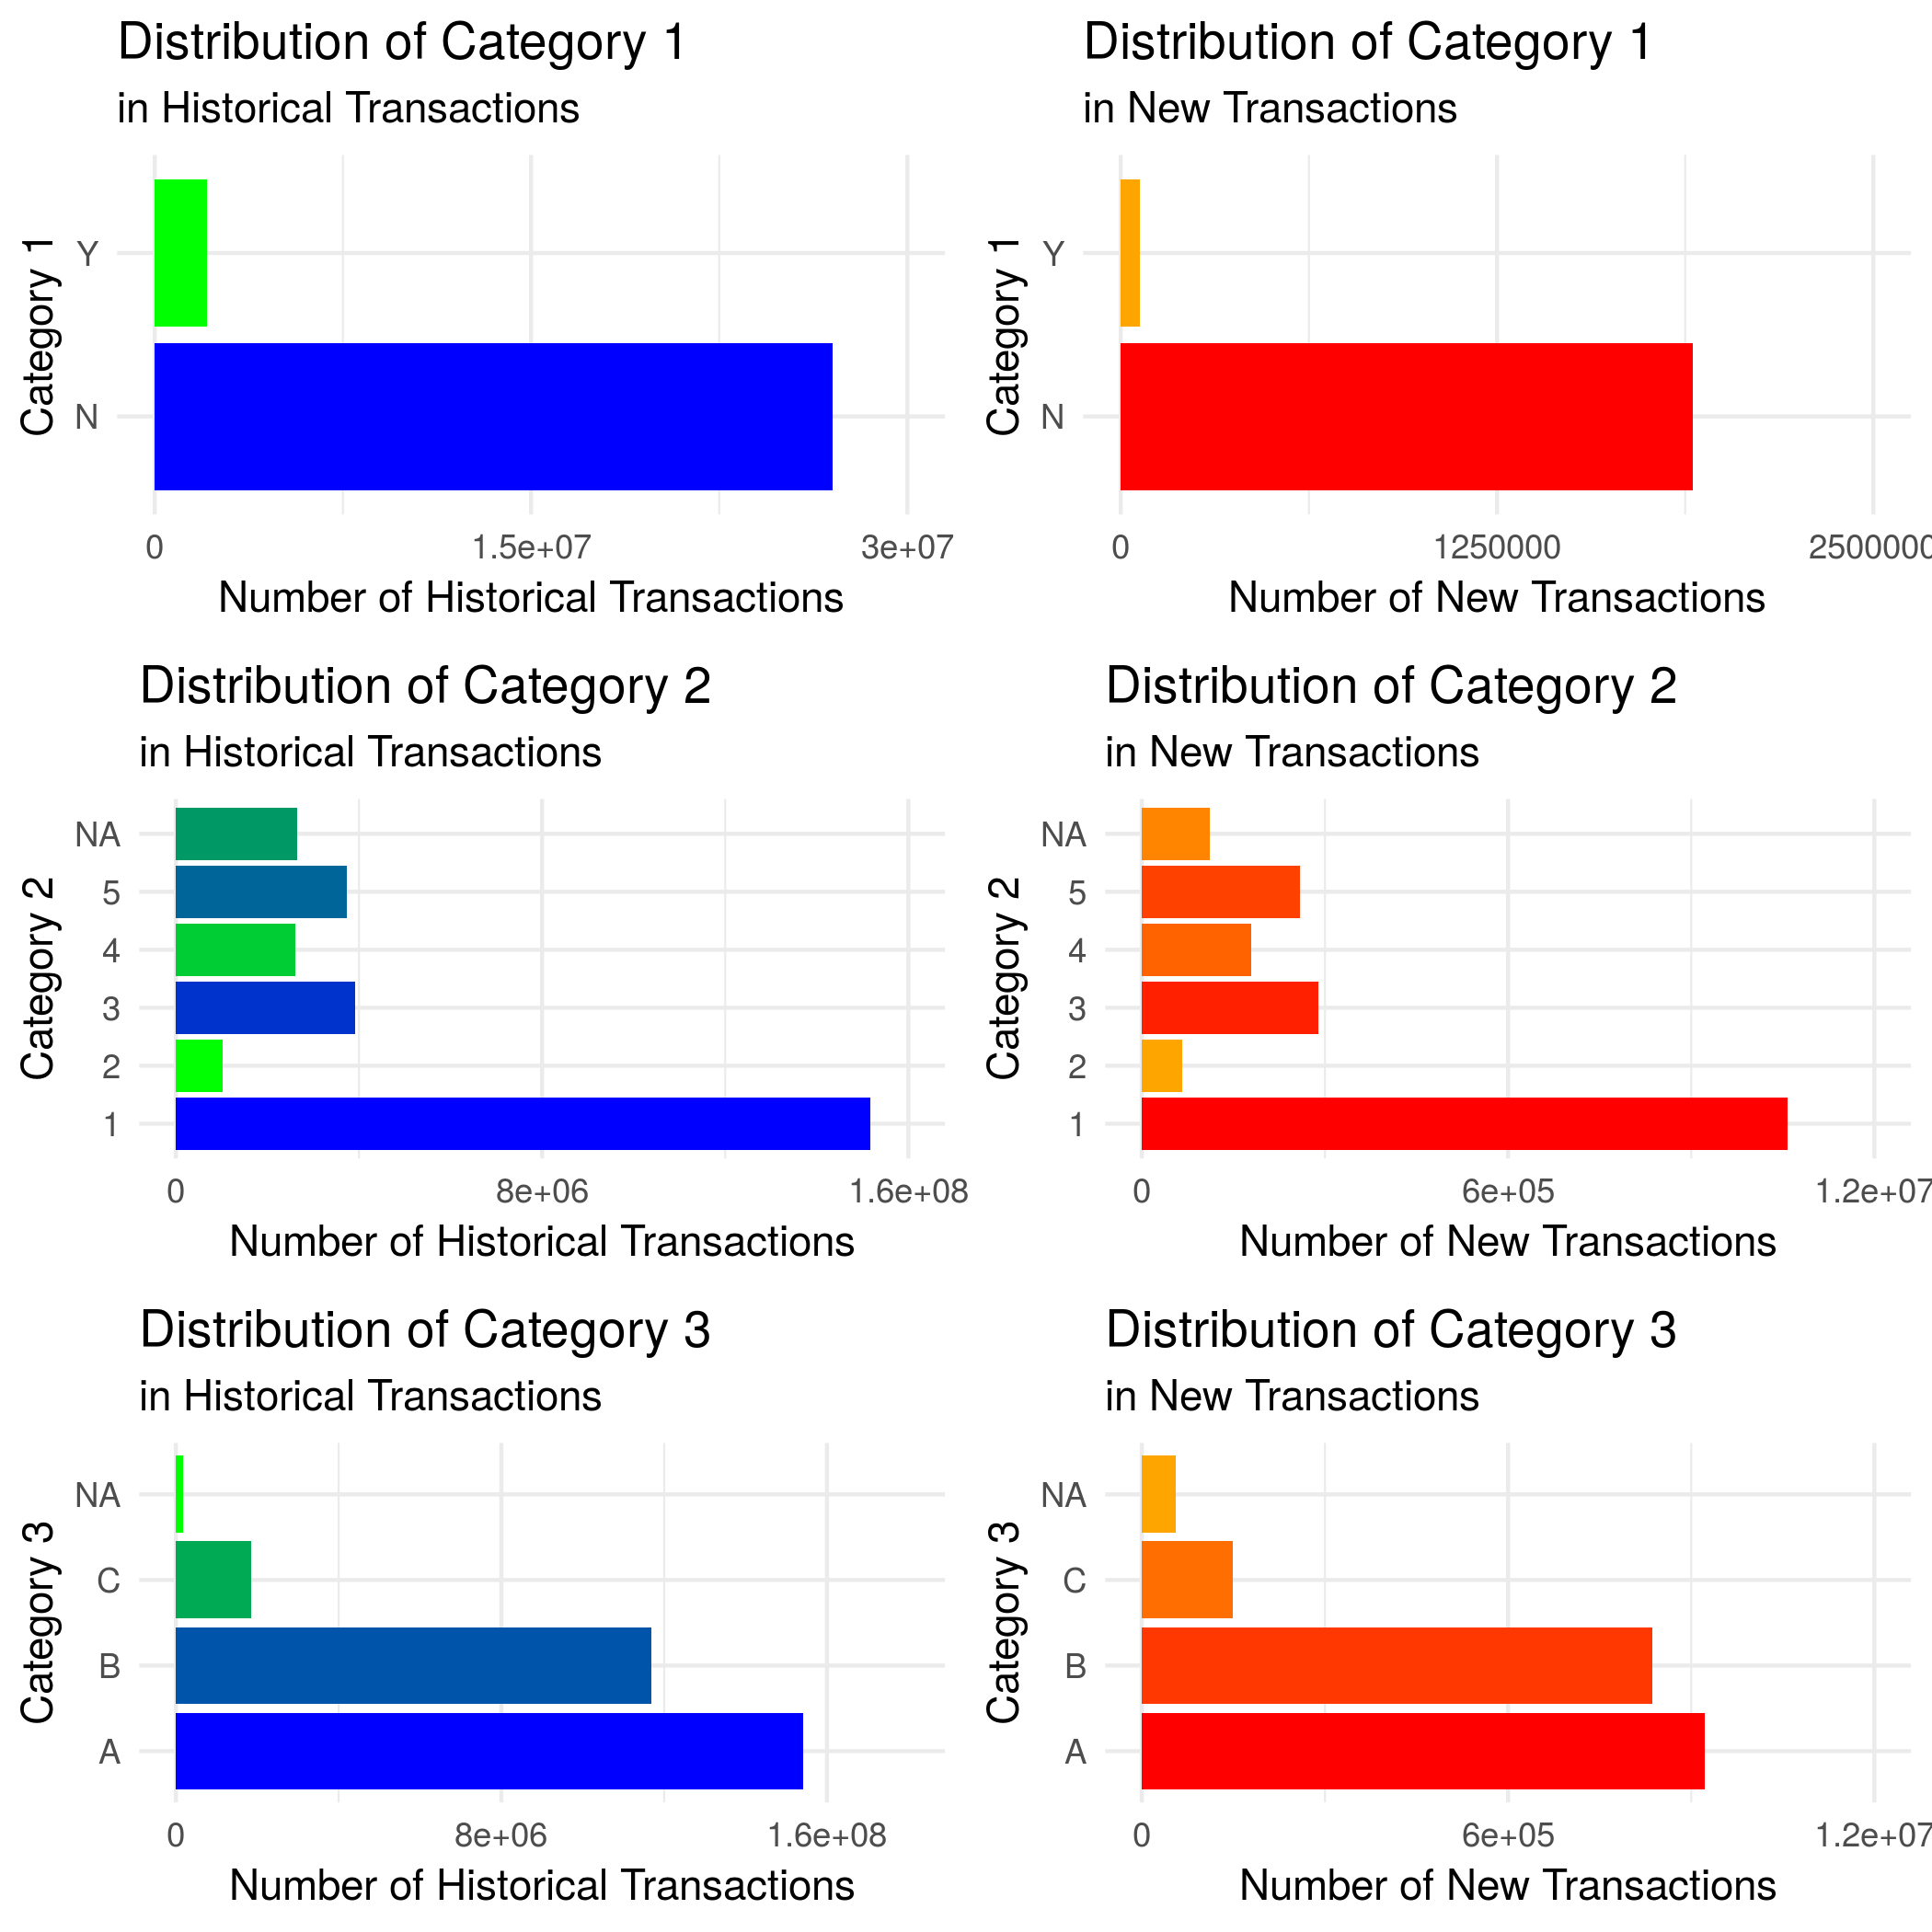
\includegraphics[scale = 0.45]{cat_plot} \caption{Distribution of categorical features in transactions data.} \end{figure} 
In Figure 5, there are a number of similarities between both types of transaction data. A value of \texttt{Yes} for category $1$ is not evident in the data for both transactions data. In fact, there are $30$ times as many records of \texttt{No} than \texttt{Yes} in the new transactions. As for category $2$, a similar analysis can be done. A value of $1$ is overly found whereas $2$, $3$, $4$ and $5$ are less likely to occur. Values $3$ and $5$ are almost similar in number of occurrences for both transactional datas. Note that there is a high number of null values, indicating missing data. It is even more than the number of $2$s in this category. Lastly, category $3$ is looked at. A value of $A$ and $B$ is hugely preferred whereas $C$ is not so evident. Missing values is also a problem for this data column. Looking at the big picture, there is no significant differences in the distribution of category values for both transactional datas. 

Now, transactional data will be examined using the purchase date feature. To extract richer information, this feature is broken into four valuable data columns: month, day, hour and bins of three months. 
 \begin{figure}[b!] 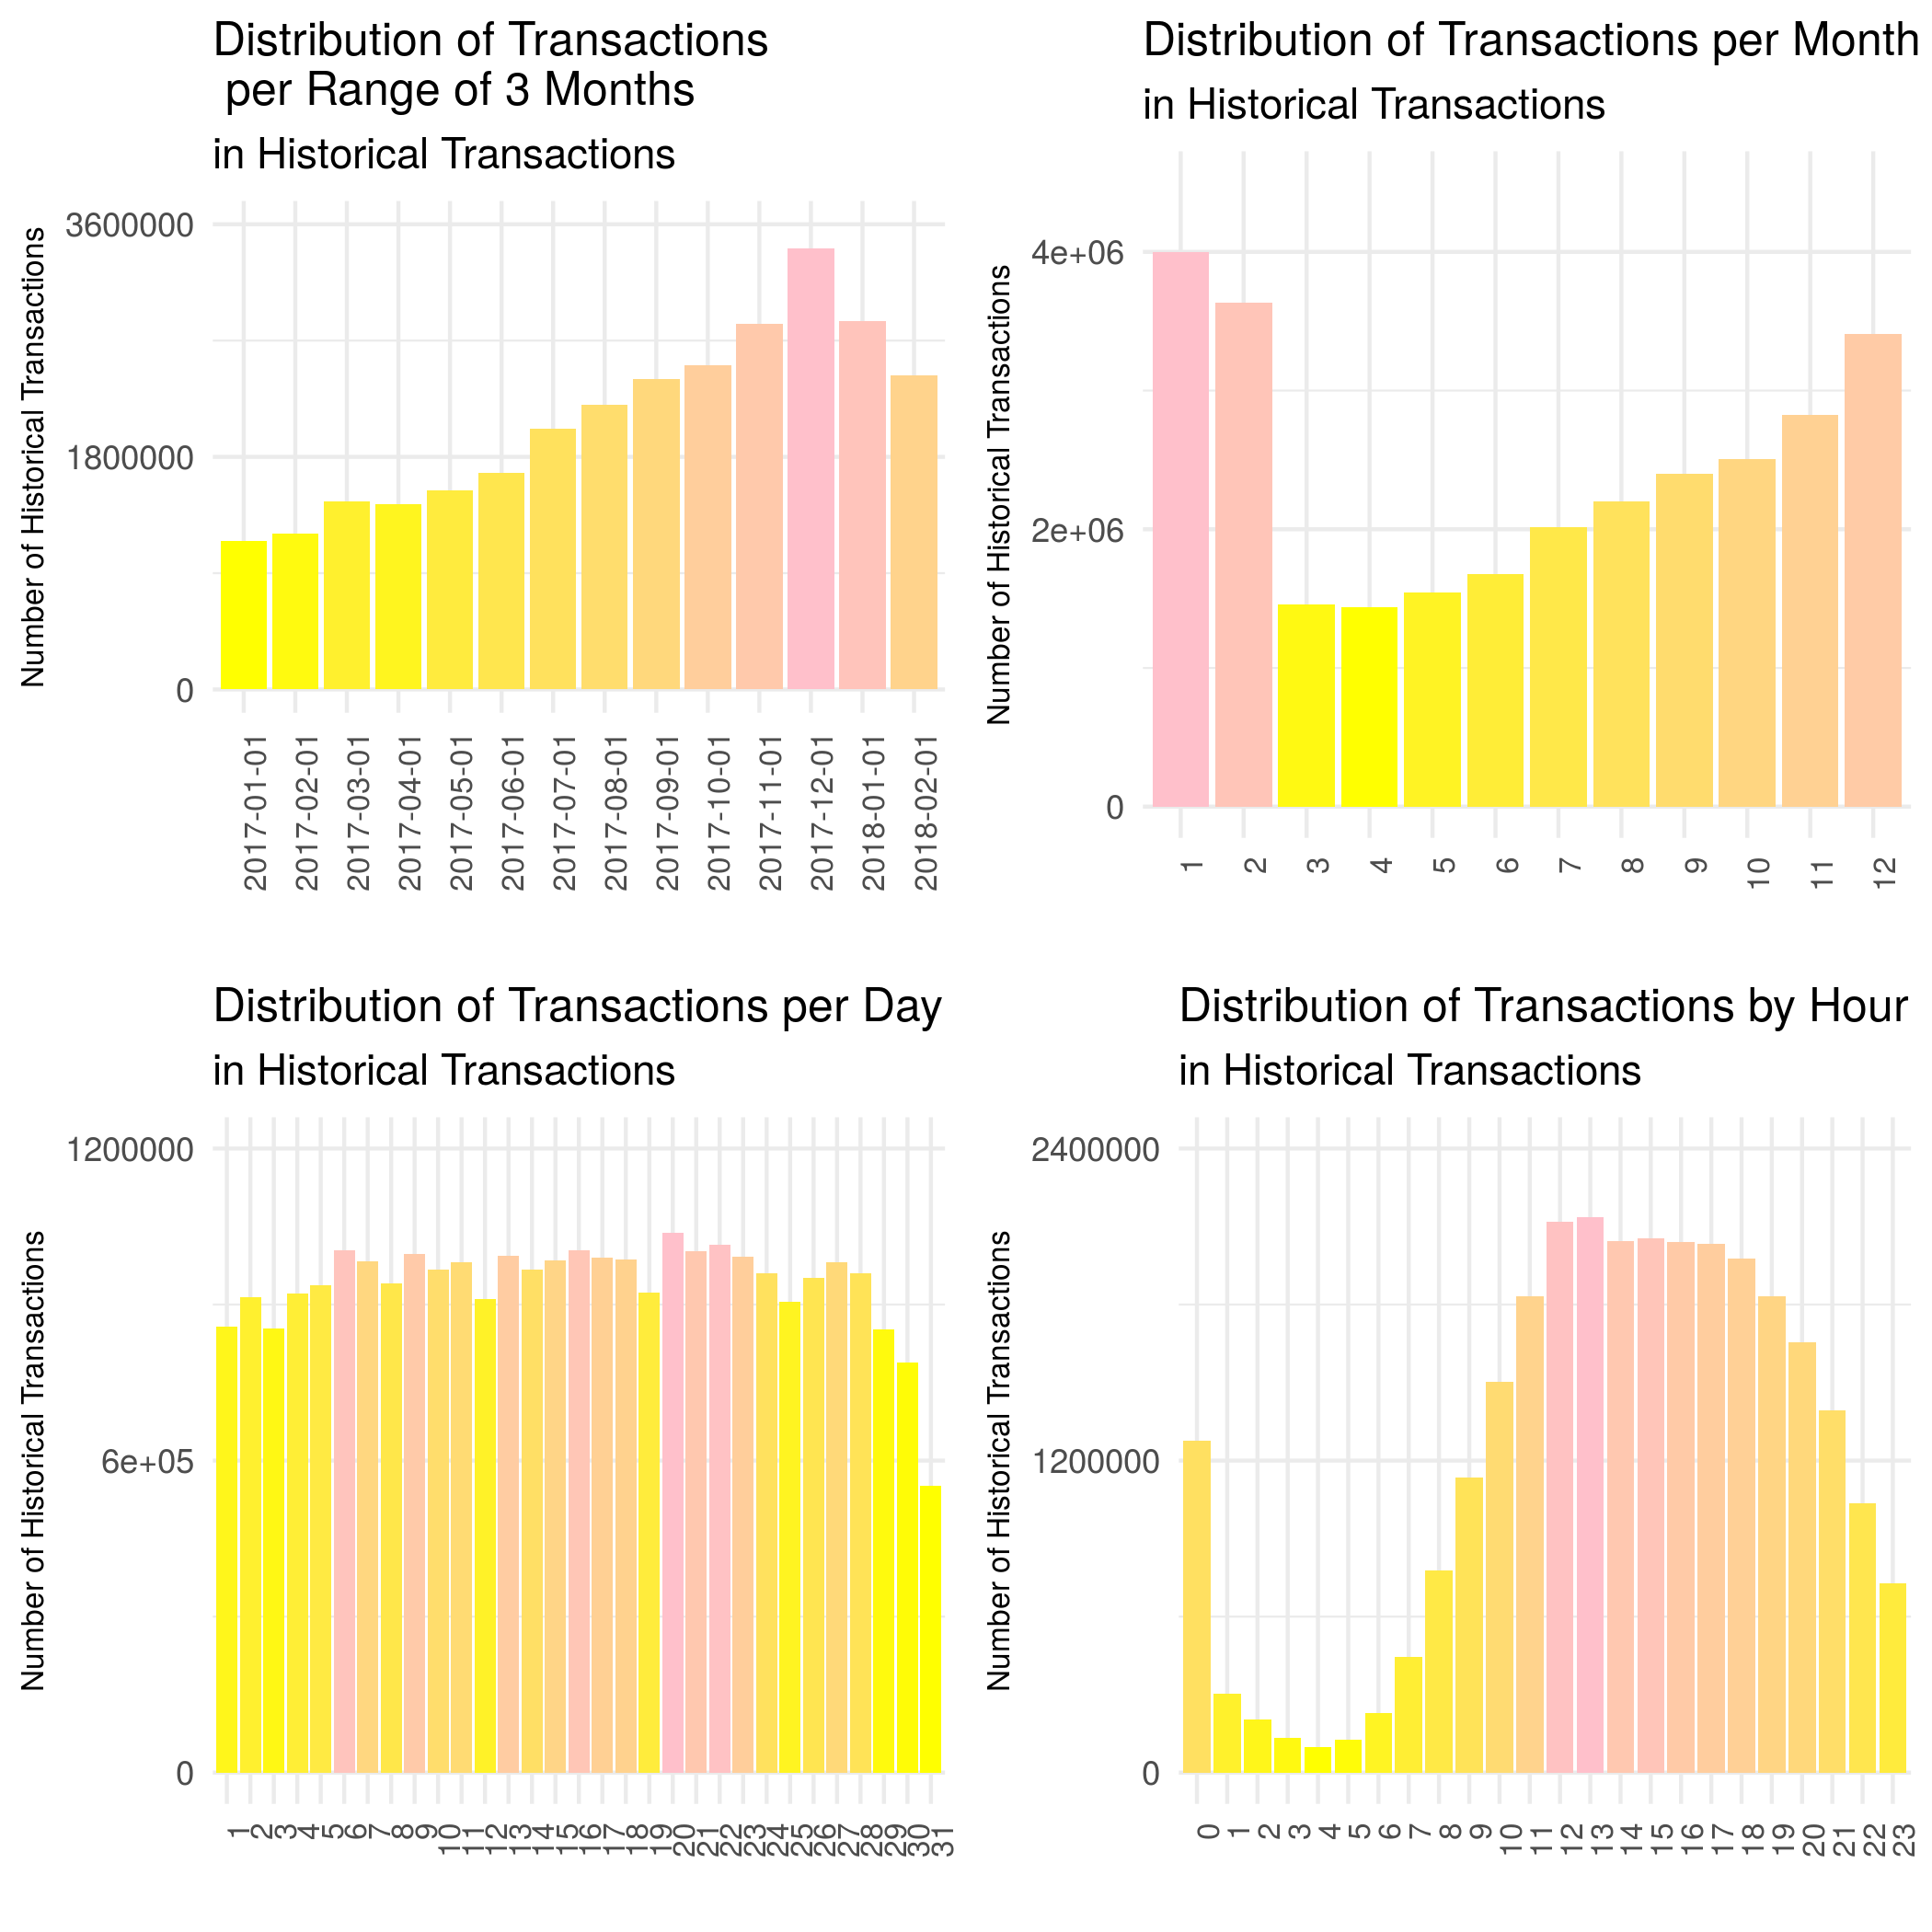
\includegraphics[scale = 0.4]{ht_time} \caption{Distribution of time of purchases in hist. transactions.} \end{figure} 
 \begin{figure}[b!] 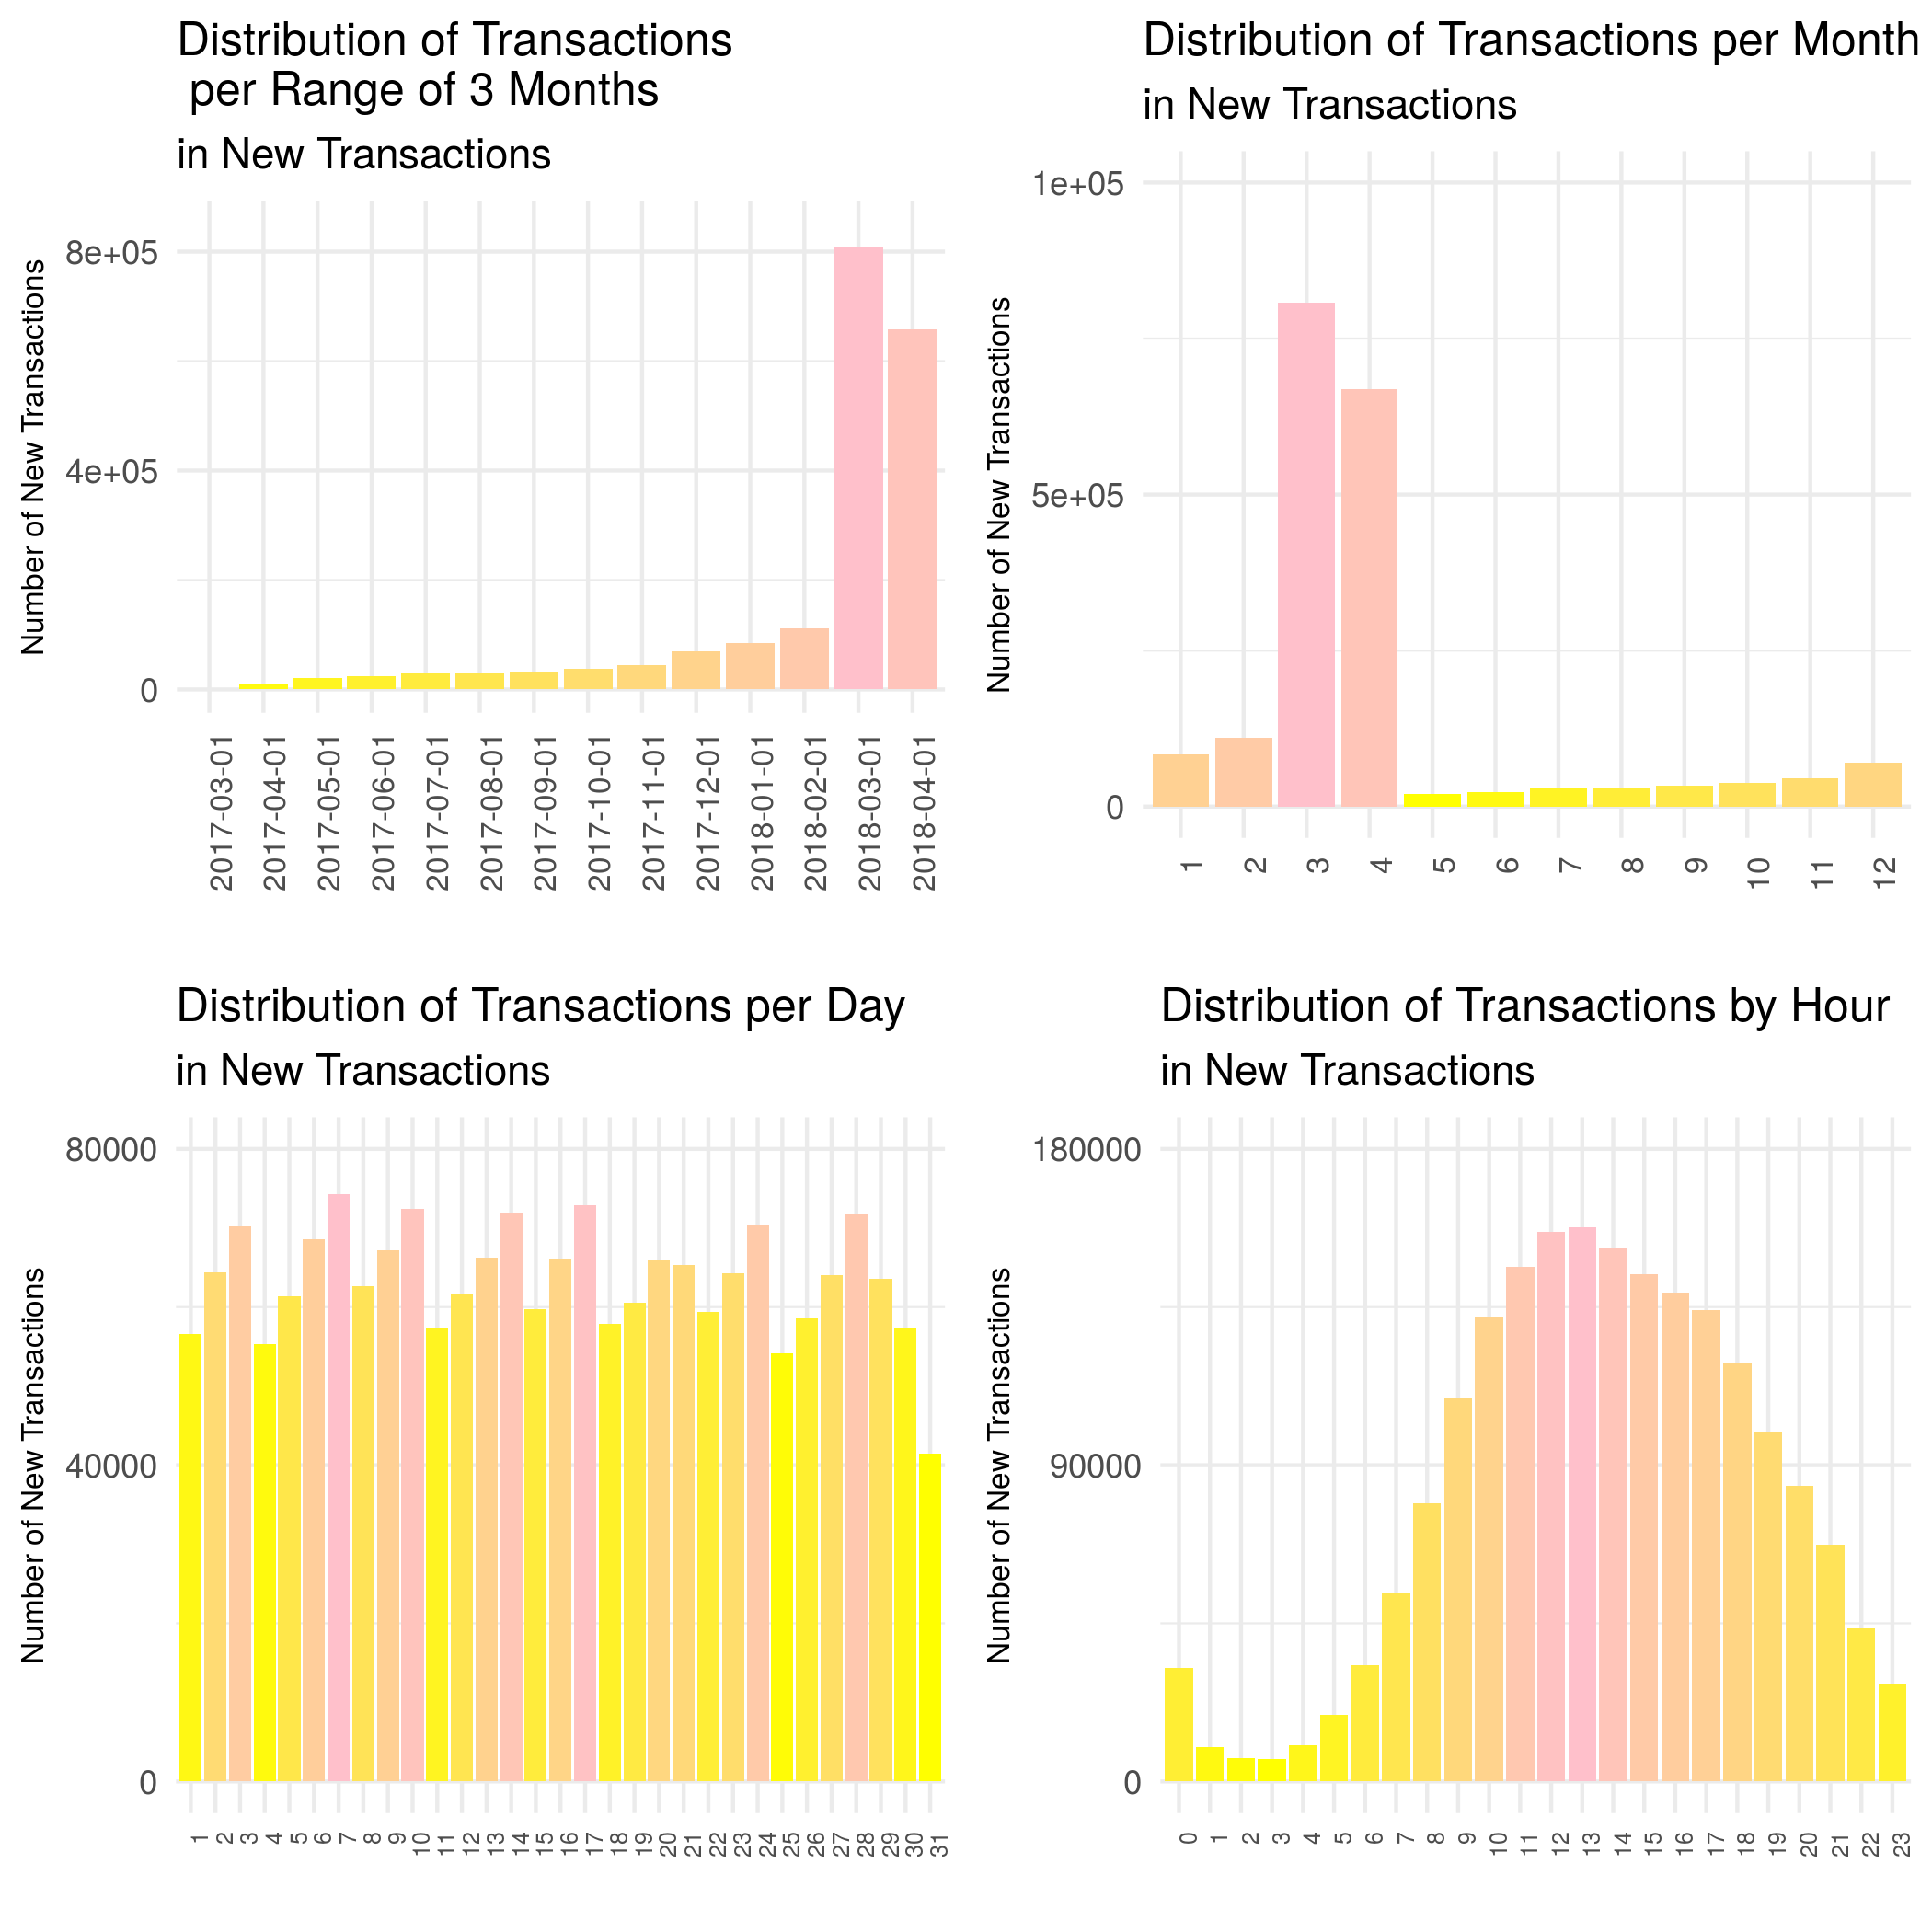
\includegraphics[scale = 0.4]{nt_time} \caption{Distribution of time of purchases in new transactions.} \end{figure} 
Several observations can be made here from Fig. 6 and Fig. 7. The number of historical transactions made every $3$ months grew gradually from January $2017$ to December $2017$ and then leveled off. This is different in the new transactions where number of transactions are really low until June $2018$ when it shoots up and then level off a bit in April. A similar pattern is noticed in the distribution of transactions by month. Number of historical transactions grew from March to February, where the highest number of transactions were made in January. This is different in the new transactions where it stayed low all year round except having an all time high in March and April. There are also interesting patterns found when looking at customer transactions by day and hour. In the historical transactions dataset, number of transactions tend to be higher in the middle of the month and lowest at the end of the month; in addition, the distribution of transactions as a function of hour is periodic. Number of transactions reach an all time low at $4$ AM and an all time high at $1$ PM, which is usually lunch time. The hourly distribution is same for the new transactions but when looking at the per day distribution, there is a strange pattern occurring. It seems to be that people make more purchases every $3$ or $4$ days and then slow down at the end of the month. It would be interesting to study why people spend less at the end of the month. In addition to looking at how people's shopping habit changes with time, it will also be useful to look at how the number of transactions made relates with individual's target/loyalty score. 
 \begin{figure}[t!] 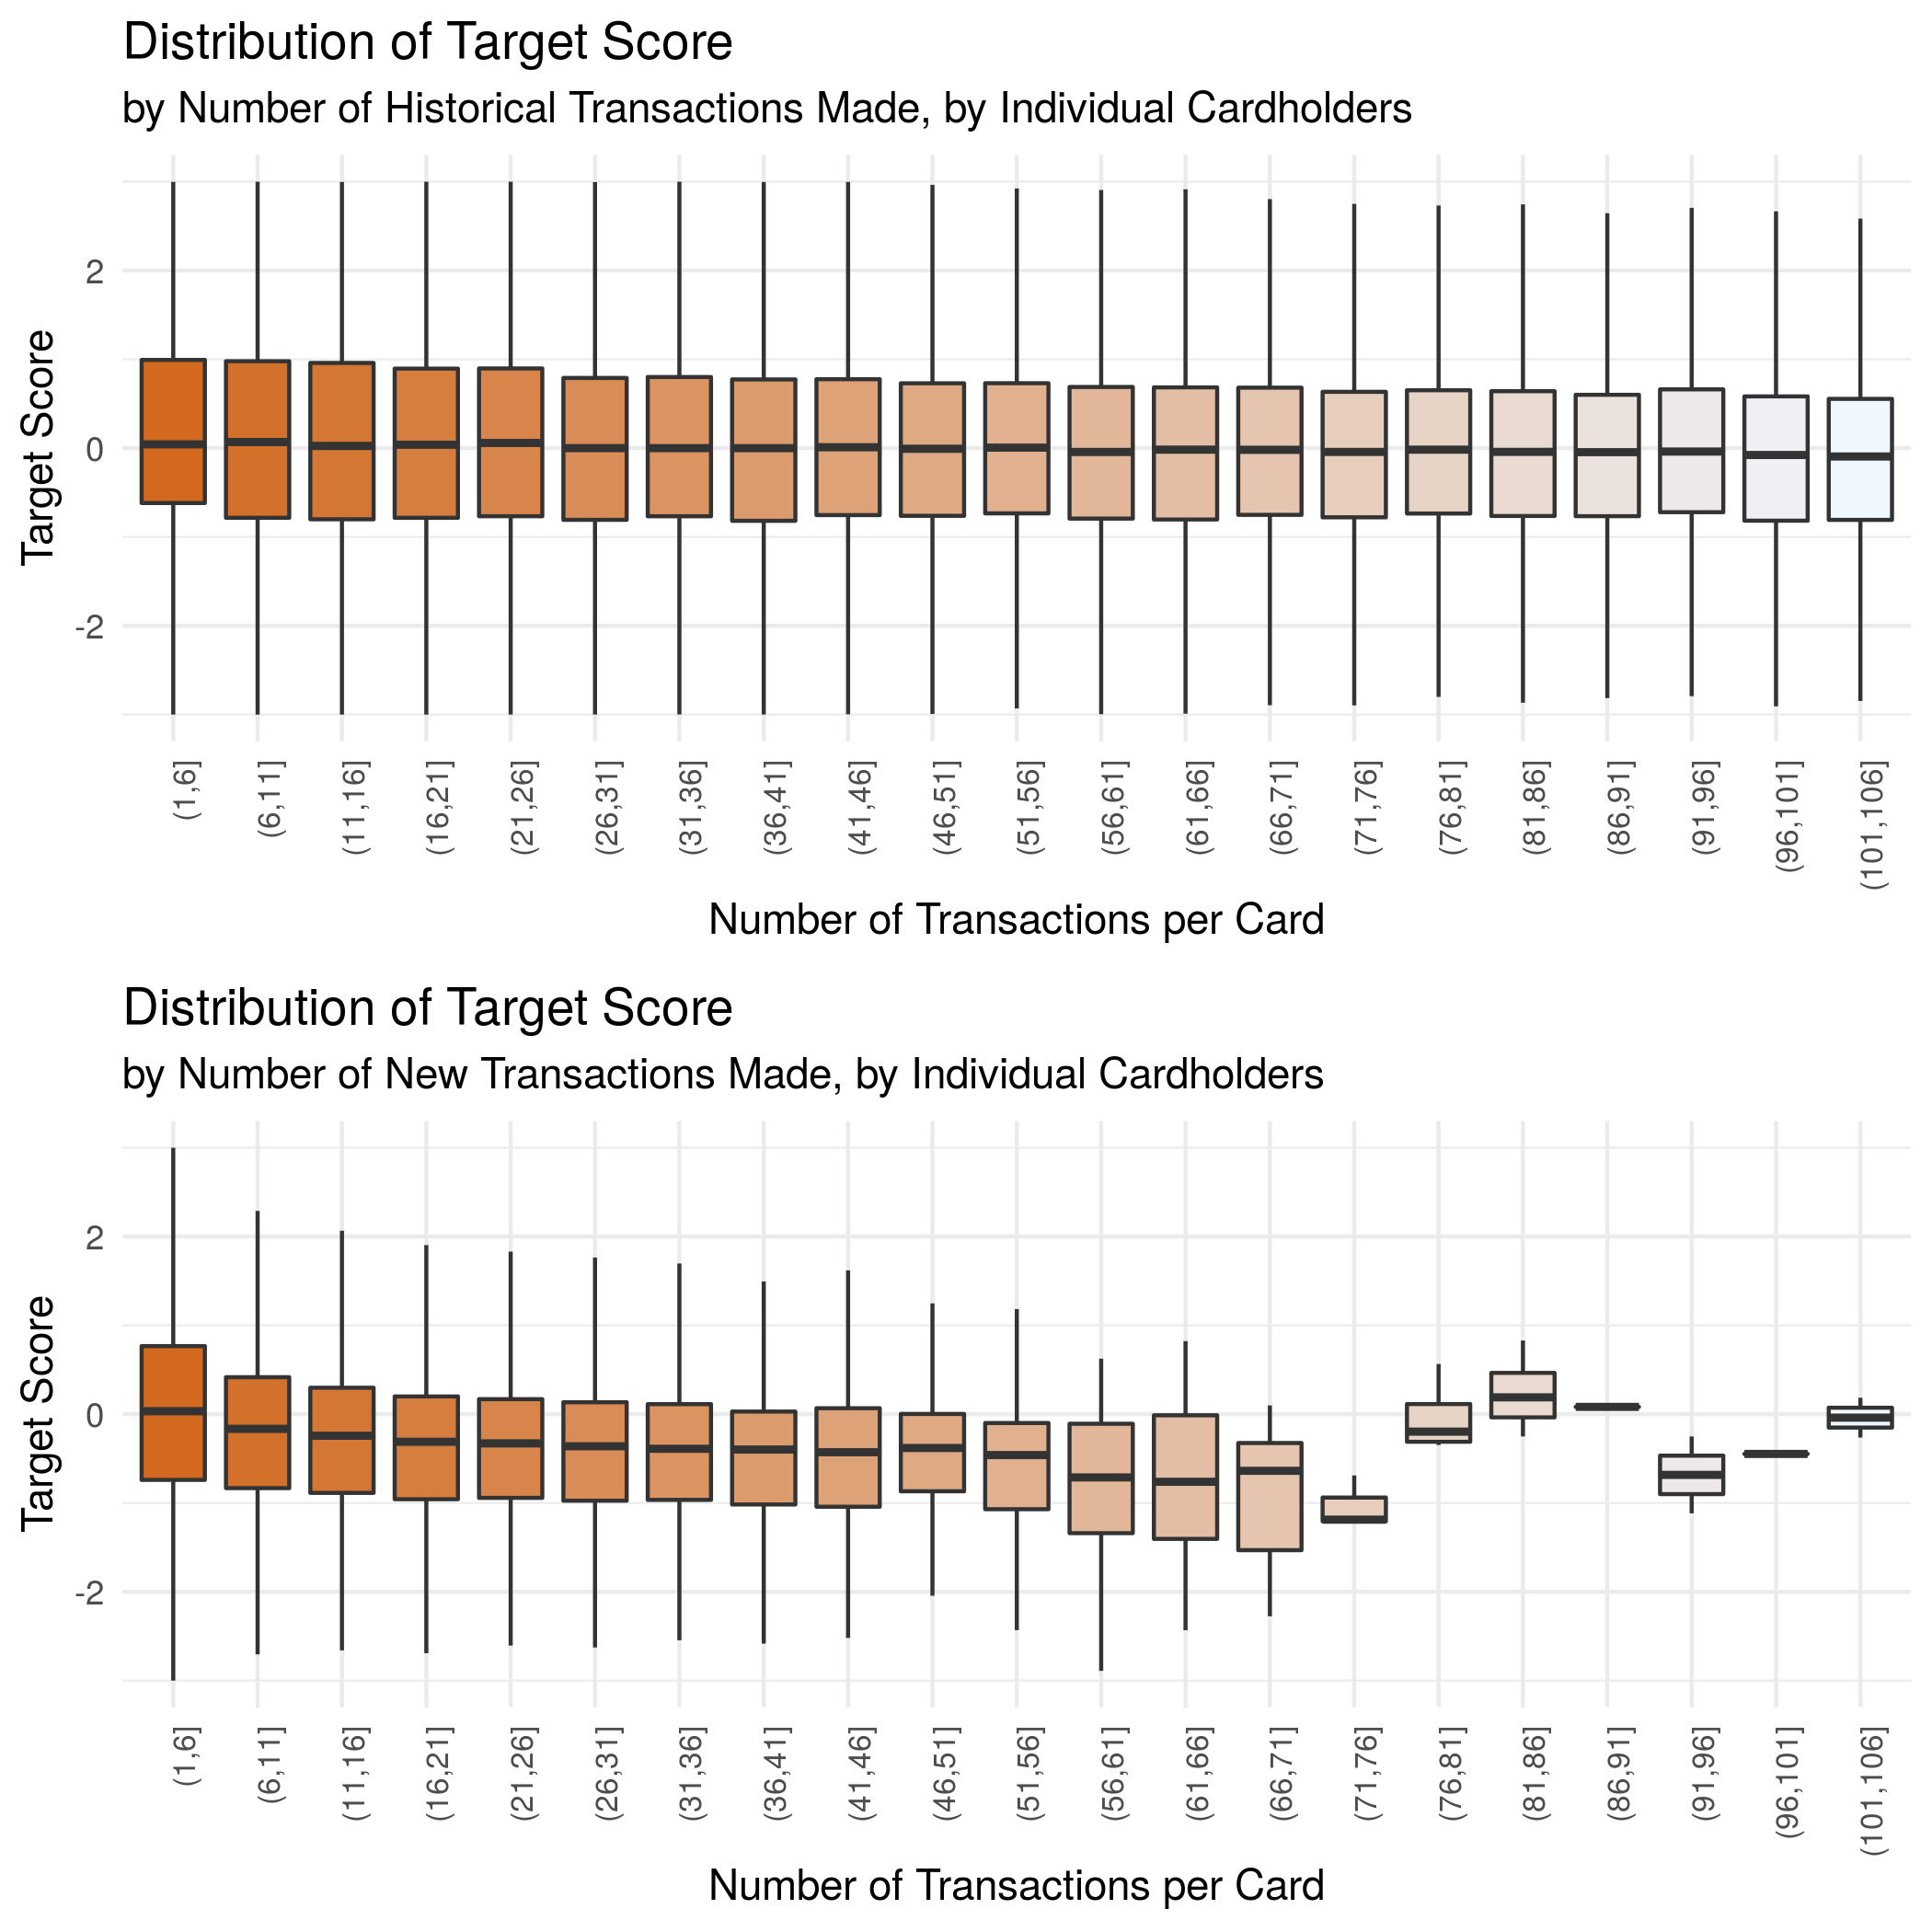
\includegraphics[scale = 0.4]{ntts} \caption{Distribution of loyalty score per binned number of transactions per card.} \end{figure} 
In Fig. 8, a series of box plots are shown depicting how the loyalty score is distributed as per each bin of number of transactions per cards in either transaction files. In the historical transactions, it is evident that as people make more and more purchases, their loyalty scores stay relatively distributed with a median of $\approx 0$. However, the third quantile, meaning the value at which $75\%$ of the scores are below this, steadily decreases from $1$ to $0.75$ when number of purchases is between $101$ and $106$. While the distribution here is relatively constant, there is a different story told with new transactions. As more purchases are made, the median loyalty score levels off from $0$ and reaches an all time low at $71$ to $76$ purchases and then behaves periodic up to $101$ to $106$ purchases. After $51$ purchases are made, the interquartile range starts to vary for each additional five purchases. This is not the case with the historical purchases. After looking at purchases made, it will be nice to look at the number of installments card holders made to pay off their purchase. 
 \begin{figure}[t!] 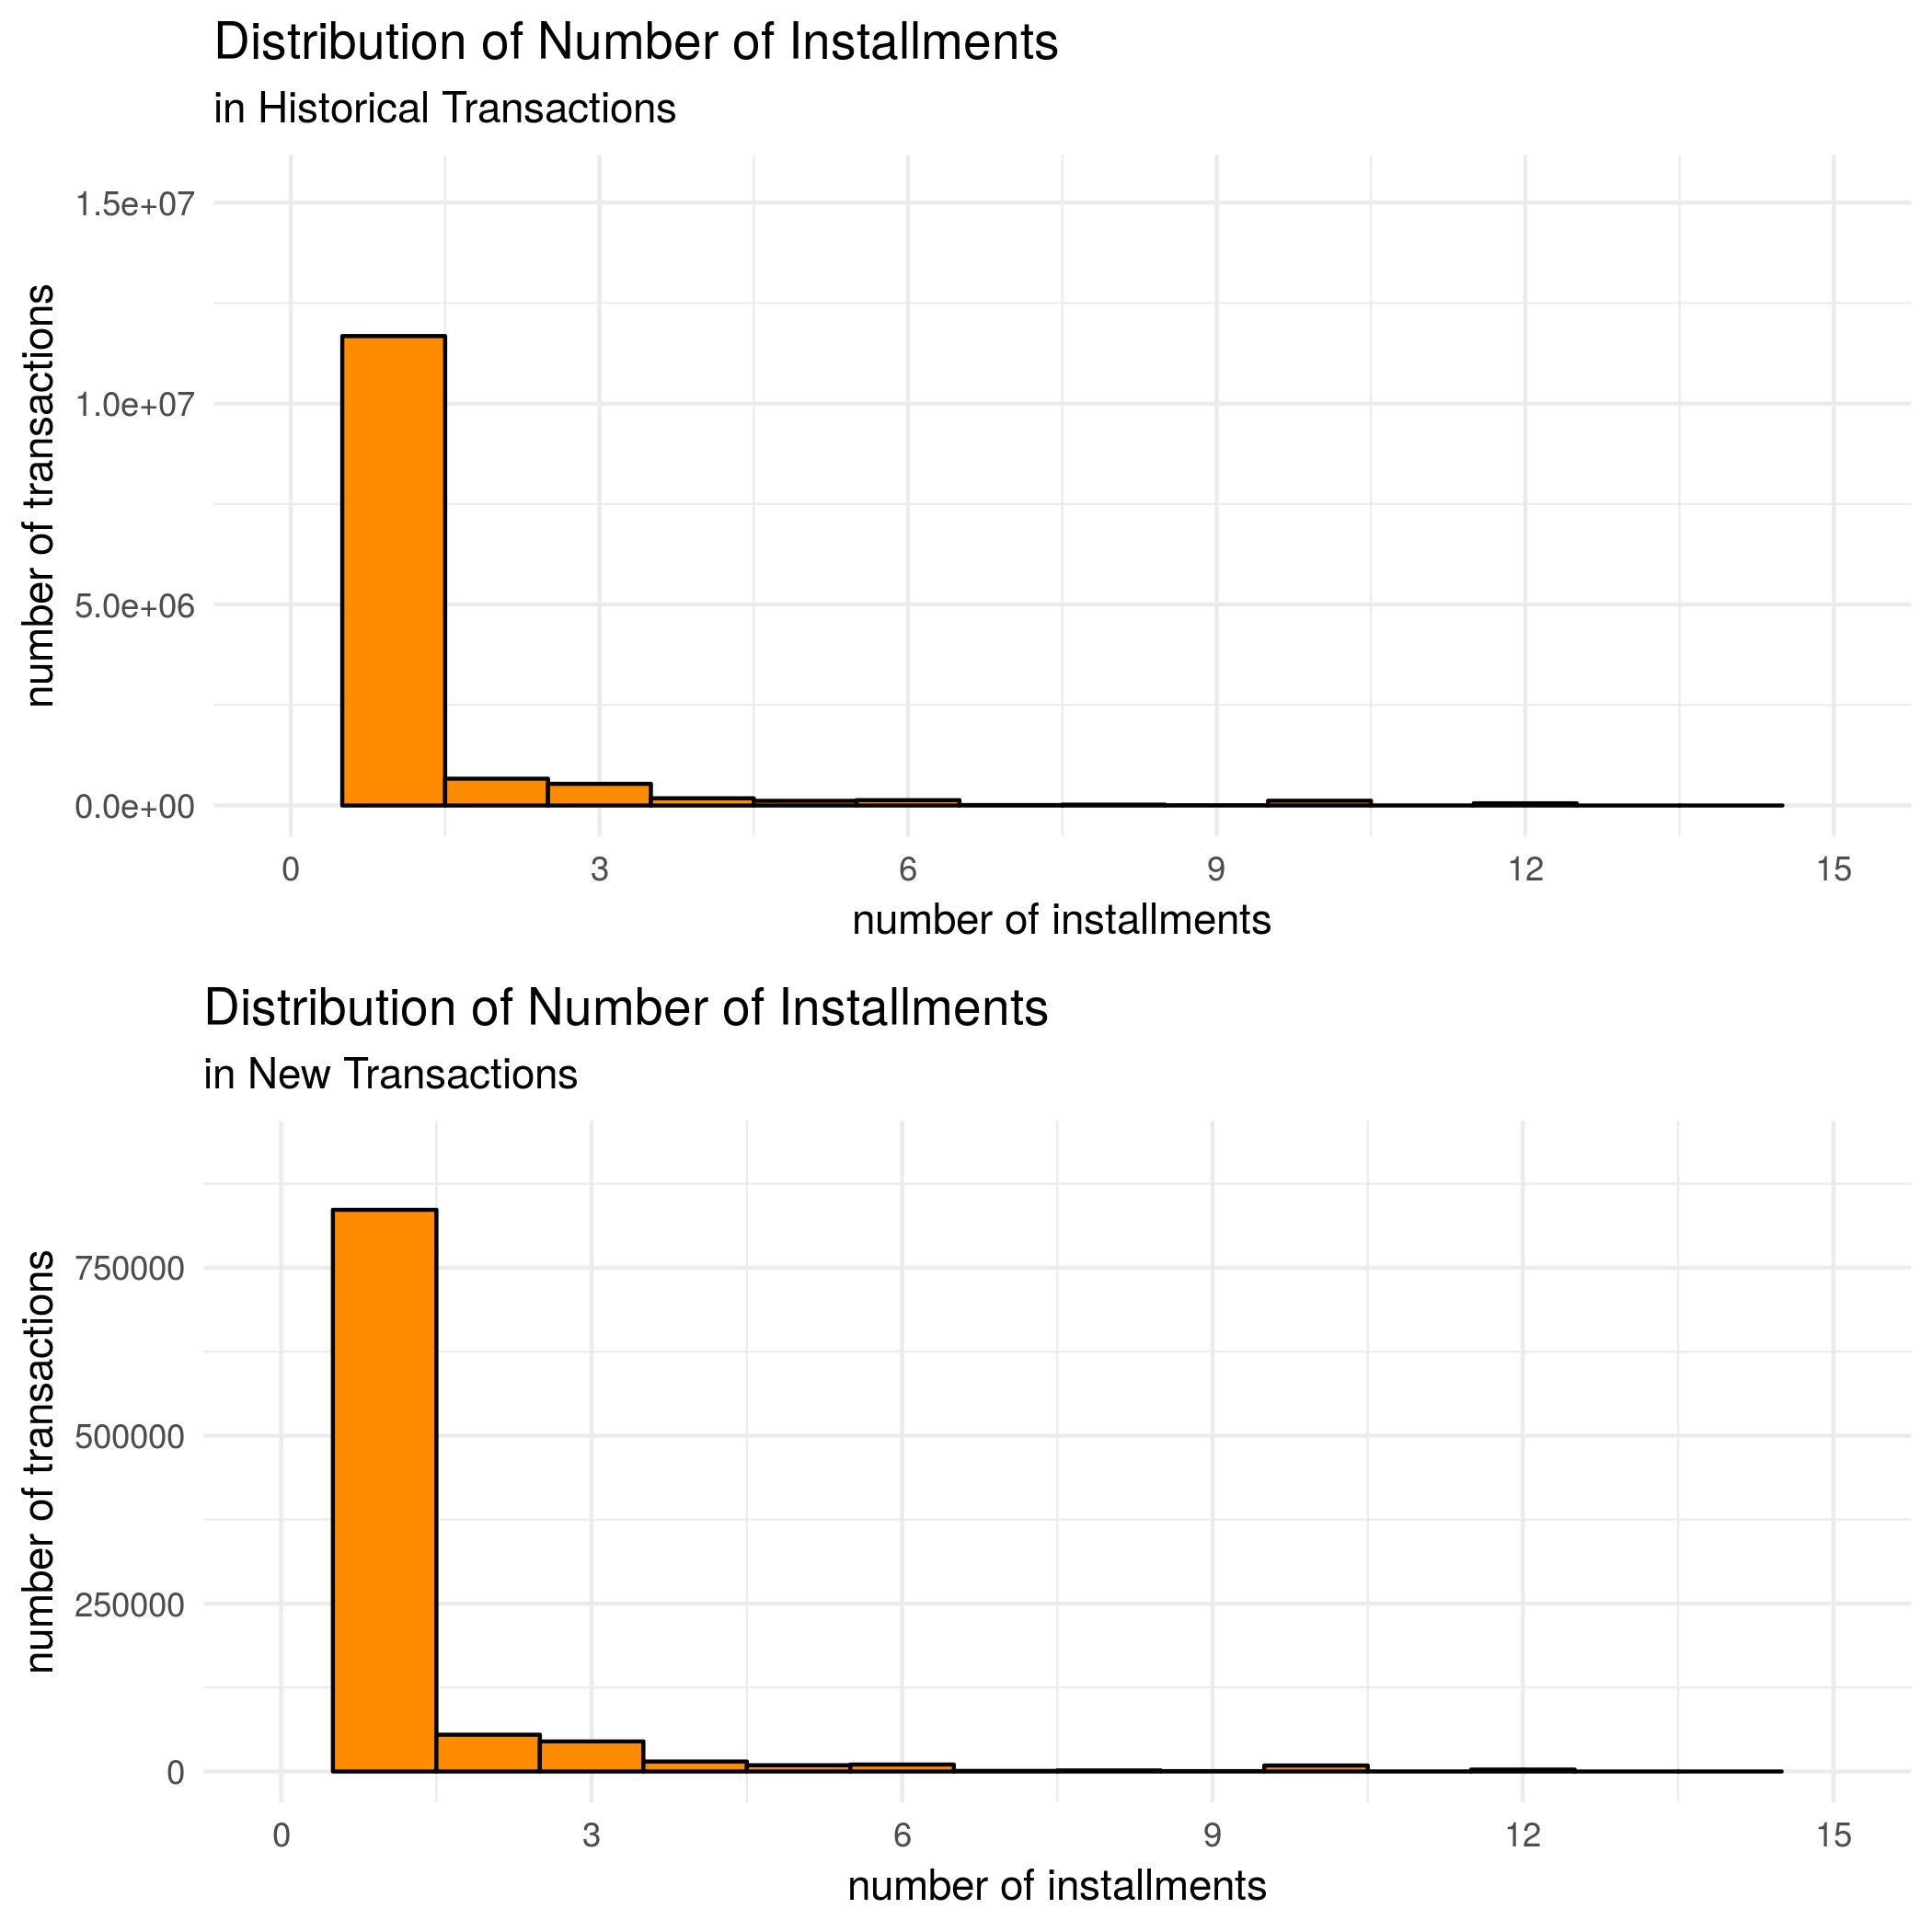
\includegraphics[scale = 0.4]{itm_count} \caption{Distribution of installments.} \end{figure} 
According to Fig. 9, it looks like patterns in number of installments people took out stayed relatively similar between both historical and new transactions. Most people only used one transactions, followed up by a small number of people making two or even three installments. There are a handful of people who have spread out their payment plan over the course of a year, or ten months. In addition, with number of installments, % latex table generated in R 3.5.1 by xtable 1.8-3 package
% Fri Apr 12 03:32:05 2019
\begin{table}[ht]
\centering
\begin{tabular}{rrr}
  
 & No & Yes \\ 
  \hline
Historical Transactions & 2516909 & 26595452 \\ 
  New Transactions & 0 & 1963031 \\ 
   \hline
\end{tabular}
\caption{Number of Authorized/Nonauthorized Transactions}
\end{table}
 it is important to see whether transactions were approved.  The number of approved and disapproved transactions are shown in the table on the left. Note that the new transactional data has no disapproved transactions. Meaning this is a constant value feature; it may not be useful for modeling. In the historical transactions, nearly $10\%$ of the transactions are disapproved. This could give insights on target scores. 

Finally, the last features that will be examined are the individual IDs. For this analysis, the top ten IDs (card, city, state, merchant, merchant category and subsector) were counted for both forms of transactions. The values are shown in Fig. 10 and Fig. 11. 
 \begin{figure}[bt] 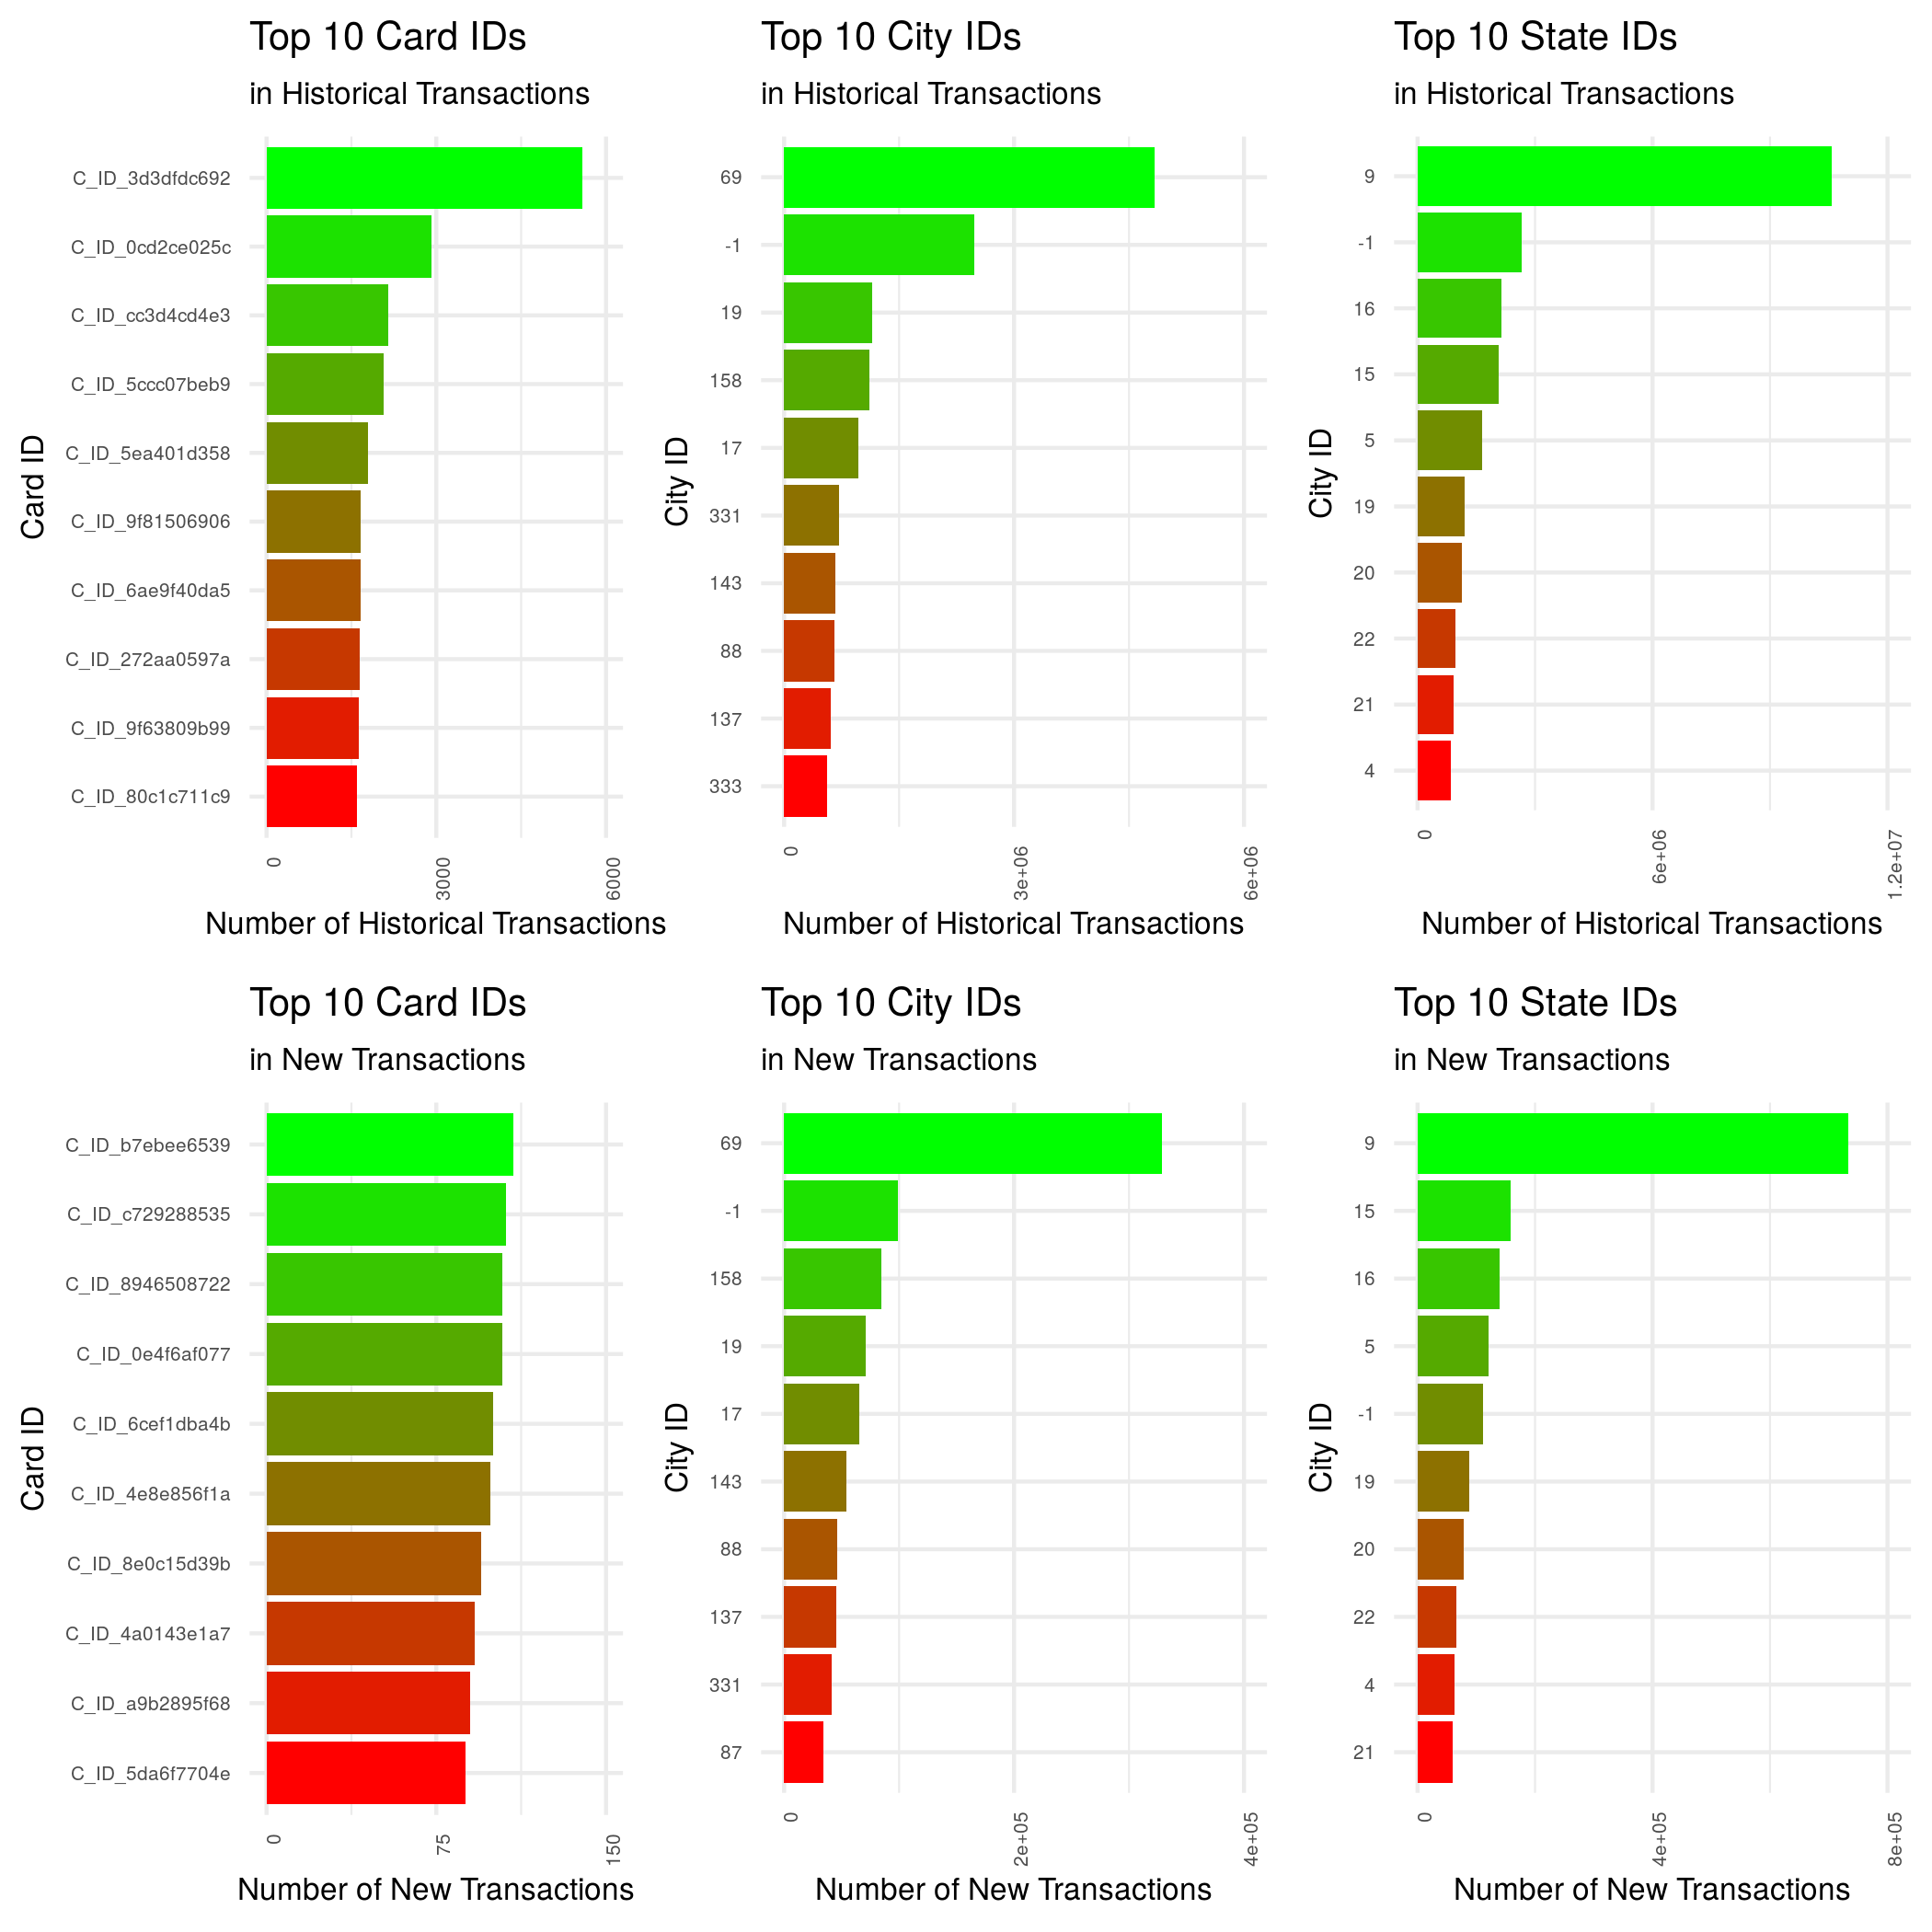
\includegraphics[scale = 0.4]{id_ccs} \caption{Distribution of card IDs, city IDs and state IDs.} \end{figure} 
 \begin{figure}[bt] 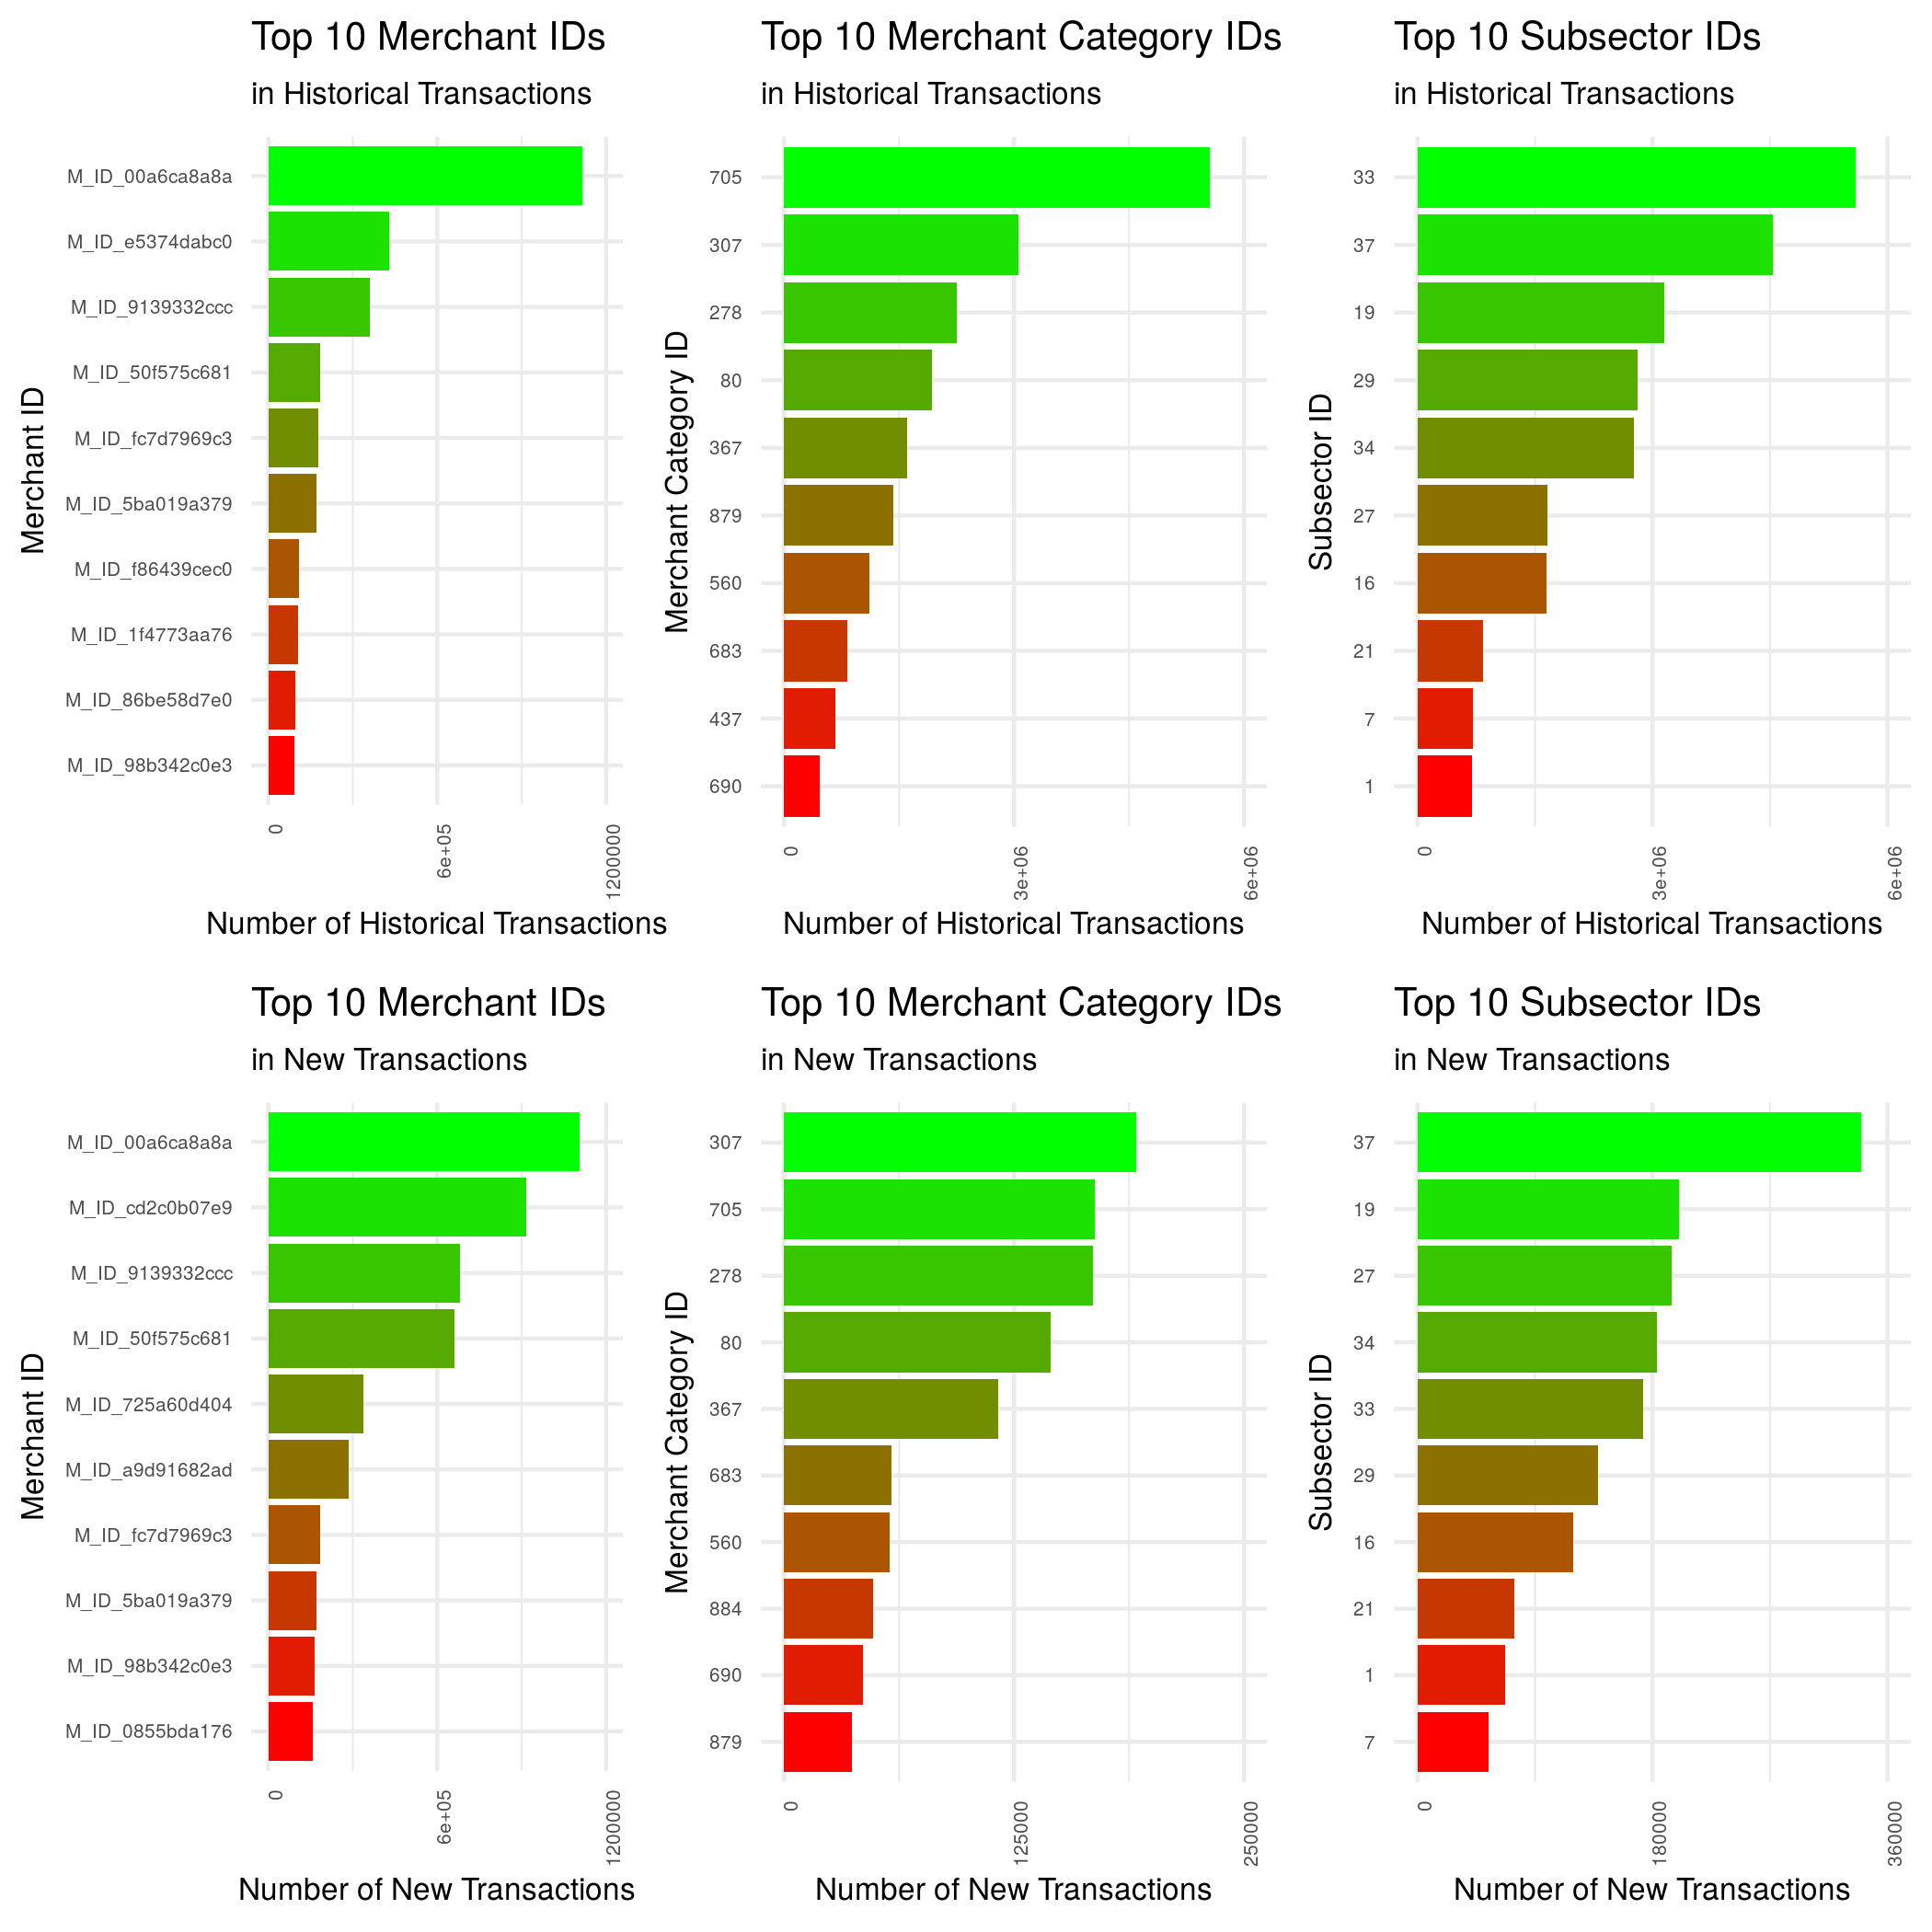
\includegraphics[scale = 0.4]{id_mcs} \caption{Distribution of merchant IDs, merchant category IDs and subsector IDs.} \end{figure} 
The key takeaways from these plots are as follows. the top ten card holders for both transactions types are different. All but one city IDs are the same in the top ten city IDs for both transaction types. The top ten state IDs are the same in both, though differently distributed. In addition, there is an existence of a $-1$ for state IDs (and city IDs); these should be dealt with later during preprocessing. Furthermore, six of the top ten merchant IDs, nine of the top ten merchant categories and ten of the top ten subsector IDs are the same for both transactional data. 

\subsection{Merchants}
In addition to transactional data, Elo has provided in depth information on different merchants that are partnered with for promotional discounts. This dataset has statistics on $334, 696$ merchants spanning $22$ variables. It shares information about merchants such as: merchant group ID, merchant category ID, merchant category group, two anonymized measures, three anonymized category data, range of revenue in last active month, range of quantity of transactions in last active month, monthly average of revenue in last three months divided by revenue in last active month, and various other numerical data on revenues and transactions in the past six months and year. For the purpose of this study, exploratory data analysis will be left out for this portion due to the high number of features to look at.

\section{Preprocessing}
Before models can be created to predict loyalty scores, the data must be put together in a coherent fashion. After all, Elo has provided a number of individual datasets to work with. It would be best to extract useful information from each dataset about each cardholder for modeling. 

\subsection{Feature Engineering and Aggregating Transactional Data}
To make use of both distinctive transactional datasets, an aggregation process will be carried out on both datasets individually. First the authorized flag column is mutated into a binary variable of $0$ or $1$ for simplicity, where $1$ represents yes and $0$ otherwise. In addition, full use of the purchase date is made again by creating new columns representing the year, month, day, hour, minute and second of purchase date. As seen in the explanatory data analysis, there are some strange values in some of the data columns, such as a $-1$ for IDs, or a record of $999$ installments. Using this information, any values for city ID, state ID, subsector ID and merchant category ID that were $-1$ were replaced with \texttt{NA}. Number of installments that were more than $12$ (exceeding a year) and less than $0$ (negative installments) were replaced with \texttt{NA}. Lastly, any normalized purchase amount that was greater than $1$ was replaced with \texttt{NA} since those were outliers. Now that all the features values are appropriate, the data can get aggregated. There are six types of aggregations done on each of the transactions data so that the transactional data only holds a row of data for each card holder. First, the number of transactions made is tallied up and stored. Then, for the authorized flag, number of installments, number of lagged months and purchase amount, the mean, standard deviation, mode, median, minimum value, maximum value and number of distinctive values is recorded. Then for the city IDs, merchant IDs, merchant category IDs, state IDs, subsector IDs, and three anonymized categories, the mode and number of distinct values is stored. Working with the derived data for purchase date, the number of distinct values, mode, minimum value and maximum value is found for the year, month, day, hour, minute and second. Lastly, using the purchase data itself, the difference between the earliest occurring purchase date and latest occurring purchase date is computed and recorded as days for each card holder. After feature engineering all these columns, the missing values in the standard deviation of the authorized flag, number of installments, number of months lagged and purchase amount is replaced with $0$. Missing values occurred because certain card holders only had one observation and thus no standard deviation was computable. At the end, the individual datasets that held these derived columns were joined together using a left join on the card ID so that all card IDs are kept safely. This process was repeated for both transactional datasets. 


\subsection{Merging Data}
Now that the transactional data is summarized and the feature engineering portion is finished, the data can be merged together. First the merchants dataset is looked at. Missing values of category $2$ are imputed with the mode. However, there are still some missing values in the average lagged sales columns. These values cannot be imputed since its values cannot be inferred from how other merchants perform, or any of the other features. Since only a maximum of $16$ merchants have missing average sales data, these merchant informations are dropped. Now, the merchant data is merged with each of the transactional data individually; the connection is made by the most common merchant ID in each of the transaction dataset and using that ID to connect the merchant's stats. Careful consideration is made so that all card holders are held, even if merchant information is not found, using a left join again. Afterwards, an overall transactions dataset is made that combined historical transactions and new transactions using the card ID, along their respective merchant information. Using this overall transactional data, the actual training and testing data is finally brought out. Each of these datasets are joined with the transactions data by card ID, making sure to only keep distinct card ID information. In addition, the first activity month column from the training/test set is formed into a numeric value as well as two addition columns of data, representing the year and month. 

\subsection{Imputation and Encoding}
The training set and test set are finally made, but they are not ready to do machine learning on. Additional steps must be taken. All the columns with data in date form are dropped. This should be safe to do since meaningful extractions were made from them when aggregating. After that, any missing values in merchant ID were replaced by the global merchant ID mode in the training set. Any other missing data was imputed using the mean or mode of the column in the training or test set. Now that all the data is represented, several of the features needed to be encoded in order for machine learning to function. For the ID mode columns, since there were thousands of distinct IDs, such as for merchants and cities, frequency encoding was used to represent the count of different IDs in numeric form rather than factored characters. This will help the machine learning algorithms learn which IDs are highly represented and which are less occurring. In addition to frequency encoding, one hot encoding was used to split categorical features into two to five binary columns that represented the value of the categories. One hot encoding was used to simplify all categorical variables as well as the most recent range of sales and purchases columns. Finally, the training and test data was in full numeric form and ready for modeling. The newly formed training ($212$ features and $201,917$ observations) and test ($211$ features and $123,623$ observations) sets were saved as .csv files for easy access later on. 

\section{Methods}
A total of ten regression algorithms will be used to make ten models in this study. These models are: 
\begin{itemize} 
\item linear regression on three original features only
\item linear regression on all features 
\item ridge regression
\item lasso regression
\item random forest
\item principal components regression
\item partial least squares 
\item $k$-nearest neighbors
\item \texttt{XGBoost}
\item \texttt{LightGBM} 
\end{itemize} 

For most of the modeling, the training data, with $201,917$ observations, will be used to train the model. The test set, with $123,623$ observations, will be used to test the model. This is a $62/38$ split. For all of these models, the model performance will be measured by the root mean squared error of the calculated loyalty scores. $$ \text{RMSE} = \sqrt{\frac{1}{n} \sum_{i=1}^n (y_i - \hat{y}_i)^2} $$ Several notes are to be made about specific models made here. For ridge and lasso regression, cross validation with $10$ folds will be used on the training data to find the best $\lambda$ parameter for the models. Using the specific $\lambda$ values, appropriate metrics will be calculated. For the random forest model, the number of trees that will be made is $25$. Furthermore, the number of variables randomly sampled as candidates at each split and the maximum number of terminal nodes in the forest will be $100$. For the principal components regression model, cross validation will be utilized again with a $10$ fold split. Metrics will be determined using the best number of components that had the lowest RMSE during cross validation. A similar technique will be applied when making the partial least squares model. The $k$-nearest neighbors model will have the parameter $k=50$, meaning that it will look for the $50$ nearest neighbors when computing the loyalty score on the test set. Note that this model will not have a training set RMSE per se due to the framework of the model but will be tested on the training data itself to attain a training set RMSE. As an added bonus to this project, two packages will be used to create gradient boosted machines. These are \texttt{XGBoost} and \texttt{LightGBM}. Both of these methods use the gradient boosted decision tree algorithm with a leaf-wise growth strategy to minimize the most loss. This is great for large datasets like in this study. The difference between these two implementations is that LightGBM is suited for fast training efficiency and better accuracy. To aid in training and testing these models, the training data will be randomly split in half to create a new training and test set. The training set will be used to train the XGBoost/LightGBM models whereas the test set will be used to calculate the test metric. Here, the XGBoost model will be made with a maximum of $500$ rounds of boosting and a maximum of $20$ rounds of training before it is stopped if the model is not improving. Additional values are also supplied for the \texttt{alpha}, \texttt{gamma}, \texttt{max\_depth} and \texttt{eta} parameters. The boosting type is specified to be \texttt{gradient boosted decision tree} and the learning rate is $0.01$. The metrics for this model will be based on the iteration that had the lowest test set RMSE. Similarly, for the lightGBM model, a maximum of $500$ rounds of boosting will be used and a maximum of $20$ rounds for when training set RMSE does not improve. Note that for any form of sampling, a seed of $2019$ will be set beforehand to maintain similarity of data points.

\section{Results}
A table of the RMSE metric is shown below for all ten models and two datasets. % latex table generated in R 3.5.1 by xtable 1.8-3 package
% Sat Apr 13 09:28:43 2019
\begin{table}[ht]
\centering 
\begin{tabular}{rlrr}
  \hline
 & Model & $\text{RMSE}_{\text{training}}$ & $\text{RMSE}_{\text{testing}}$ \\ 
  \hline
1 & Linear Regression (3) & 3.84997 & 3.81445 \\ 
  2 & Linear Regression (all) & 3.77231 & 3.73939 \\ 
  3 & Ridge Regression & 3.77288 & 3.74032 \\ 
  4 & Lasso Regression & 3.77296 & 3.73982 \\ 
  5 & Random Forest & 3.67884 & 3.70221 \\ 
  6 & PCR & 3.77231 & 3.73940 \\ 
  7 & PLS & 3.77282 & 3.73960 \\ 
  8 & KNN & 3.76842 & 3.80262 \\ 
  9 & XGBoost & 3.58933 & 3.68002 \\ 
  10 & LightGBM & 3.55860 & 3.68096 \\ 
   \hline
\end{tabular}
\end{table}
 \\
\indent A number of observations can be made here. A few models performed much better than the rest. The two linear regression models had a lower test set RME than the training set RMSE. This is interesting because error on unseen data is usually greater than error on seen data. When incorporating all the features from the transactions and merchants data, error goes down. The ridge and lasso regression models performed slightly worse on the training and testing set, compared to the linear regression models. Between the lasso and ridge, the lasso model performed better on the unseen data. This indicates that when allowing some of the coefficients to equal zero, the prediction accuracy is enhanced. In equation terms, the criterion for the ridge regression model is $$ \sum_{i=1}^n \left(y_i - \beta_0 - \sum_{j=1}^p \beta_jx_{ij} \right)^2 + \lambda \sum_{j=1}^p \beta_j^2  = \text{RSS} + \lambda \sum_{j=1}^p \beta_j^2 $$ where $\lambda$ is a tuning parameter, found by cross validation in this case. The shrinkage penalty is $\lambda \sum_j \beta_j^2$. On the other hand, the criterion for the lasso regression model is $$ \sum_{i=1}^n \left(y_i - \beta_0 - \sum_{j=1}^p \beta_jx_{ij}\right)^2 + \lambda \sum_{j=1}^p \abs{\beta_j} = \text{RSS} + \lambda \sum_{j=1}^p \abs{\beta_j} $$ Here the shrinkage penalty is $\lambda \sum_j \abs{\beta}$. Since the dataset had hundreds of features, making some of their coefficient estimates equal to zero was helpful. Now, the $k$NN algorithm was one of the worst performing algorithms. Although it had a ``fake" training RMSE of $3.76842$, lower than all the other model, it performed second worst on the testing set compared to three of the four regression models. The base linear model on the three features only was the only model that performed with greater error. This makes sense since feature $1$, feature $2$ and feature $3$ had low dimensionality. 

The principal components regression and partial least squares model performed similarly to the ridge/lasso models. Both model has a slightly better test set RMSE than both ridge and lasso. The PCR model performed slightly worse than the linear regression model, only a $0.00001$ difference in testing RMSE. A plot of the number of components in PCR and in PLS and RMSE performance is showed below in Figure 12.  \begin{figure}[h] 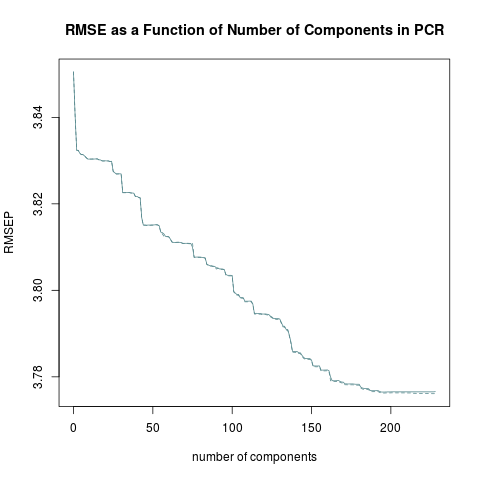
\includegraphics[scale = 0.3]{pcr_components} 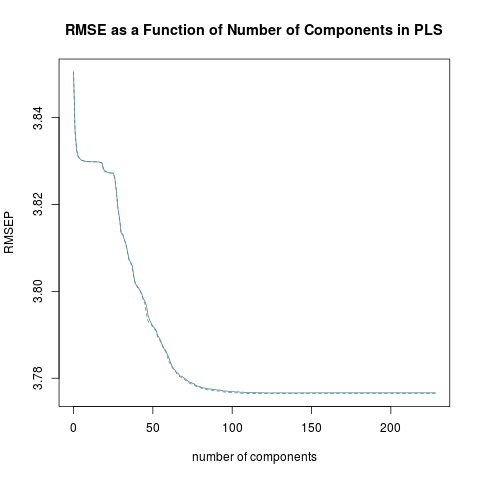
\includegraphics[scale = 0.3]{pls_components} \caption{RMSE performance as a function of components in PCR and PLS model.} \end{figure} In the PCR model, it takes at least $150$ components to explain the directions in the predictors before RMSE error stabilizes. This contrasts with the PLS model where the loyalty score was used to explain the directions in the predictors. Now, about $80$ components will give the lowest RMSE score in the cross validation phase before it just remains there as more components are added. This is why $150$ and $80$ components are used to predict loyalty scores in the test set for respective models. A con for using these two algorithms is that it runs very slow on high dimensionality data, as was evident when creating the models here even when using AWS. 

Trees are amazing. They are easily interpretable and they perform variable selection. The random forest model with $25$ trees gave a new all time low training error of $3.67884$ and test error of $3.70221$. It is the best performing model so far. A plot of the top $30$ important features found by the random forest algorithm is shown below in Fig. 13. \begin{figure}[ht] 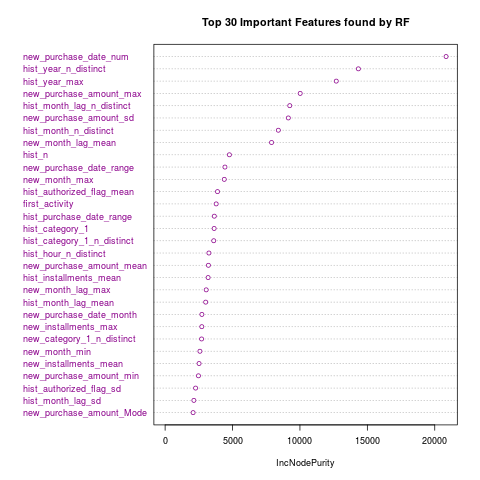
\includegraphics[scale = 0.4]{rf_features_plot} \caption{Important features determined by the random forest algorithm} \end{figure} The most important feature found was the purchase date from new transactions in numeric form. Whether transactions were made in $1$ or $2$ years in the historic transactions was next in line in terms of importance followed by the maximum year value in historical transactions. The number of historic transactions made by each card holder is in $9$th place. The one for new transactions is not in the top $30$. This features from the historic transactions make up slightly less than half the top $30$ important features. Purchase date, purchase amount and month informations are very important features. It paid off to feature engineer them and remove errors in data collection. 

The XGBoost model performed even better than the random forest. It has an all time low training set RMSE of $3.58933$ and test set RMSE of $3.68802$. This shows that boosting trees using gradients can be even more effective on performance accuracy. A plot of the RMSE as the model is trained is shown in Fig. 14. \begin{figure}[h!] 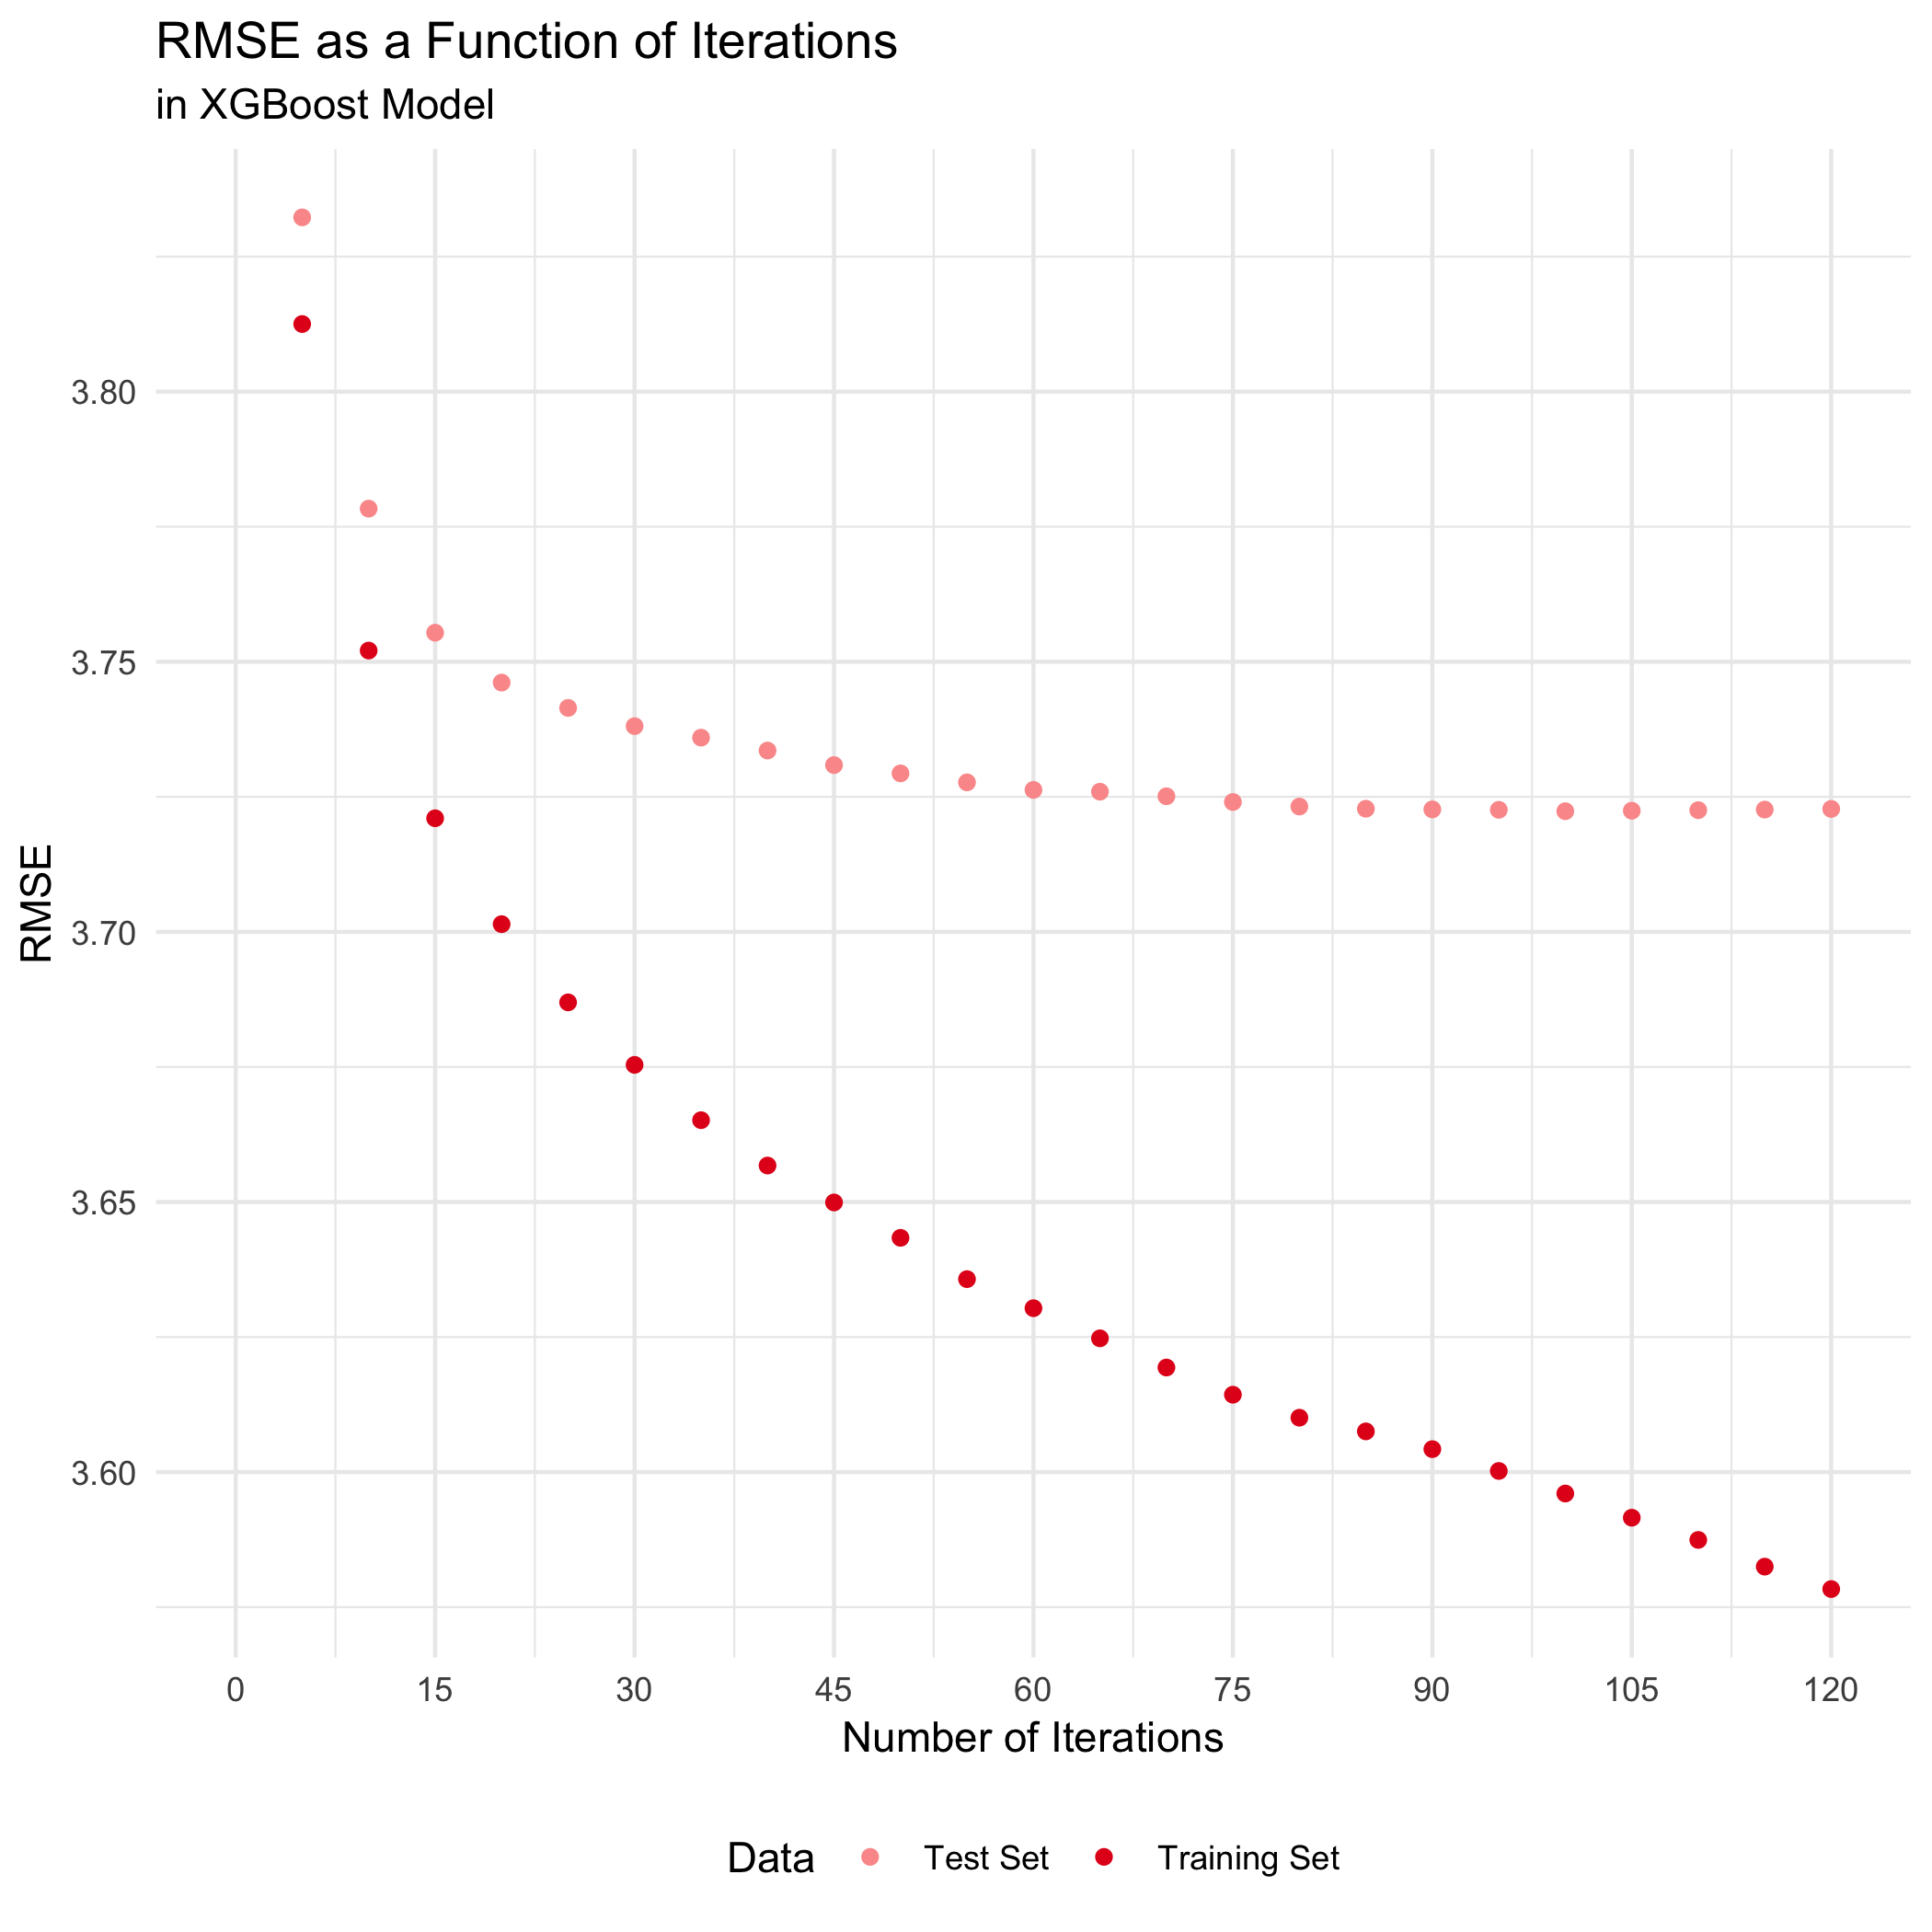
\includegraphics[height=7cm, width=7cm]{xgb_rmse} \caption{RMSE as a function of iterations in XGBoost.} \end{figure} Too many iterations do not show to be effective for generalizing the model. After $60$ iterations, the test metric does not appear to improve by a whole lot even though the model is learning more from the training set. However it does not indicate any sense of overfitting since the test error does not go up. A visualization of the top $30$ important features determined by the algorithm is shown in Fig. 15. \begin{figure}[h!] 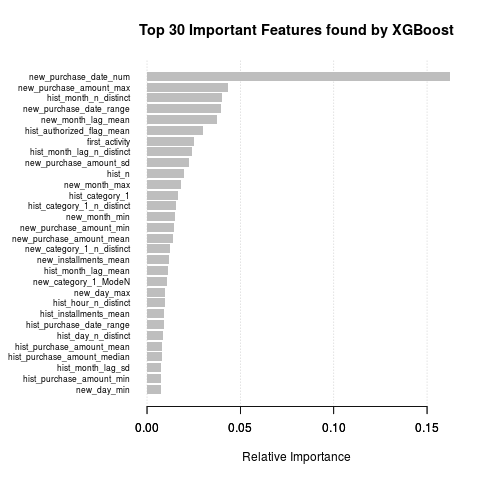
\includegraphics[scale = 0.4]{xgb_features_plot} \caption{Important features determined by the XGBoost algorithm} \end{figure} There is a different collection of top $30$ important features here. Even though the one at position one stayed the same, the second place is now taken over by the maximum purchase amount a card holder has made in new transactions. This is now followed up with the number of different months they have had a transaction. Furthermore, the number of historic transactions made by each card holder is in $10$th place. There are more historical transactions features that are deemed valuable now than in the random forest model. The time for first activity for each card holder is now more important than in the previous model. This was one of the original data piece from the original training set, only formatted into a numeric form. 

The final model that was created was the LightGBM model. It trained even better, having an RMSE of $3.55860$, whereas the training RMSE for XGBoost was $3.58933$. The test metric was slightly higher than that for XGBoost, by $0.0009$. It is still the second best model in terms of validation performance. A plot of the RMSEs is shown in Fig. 16. \begin{figure}[t] 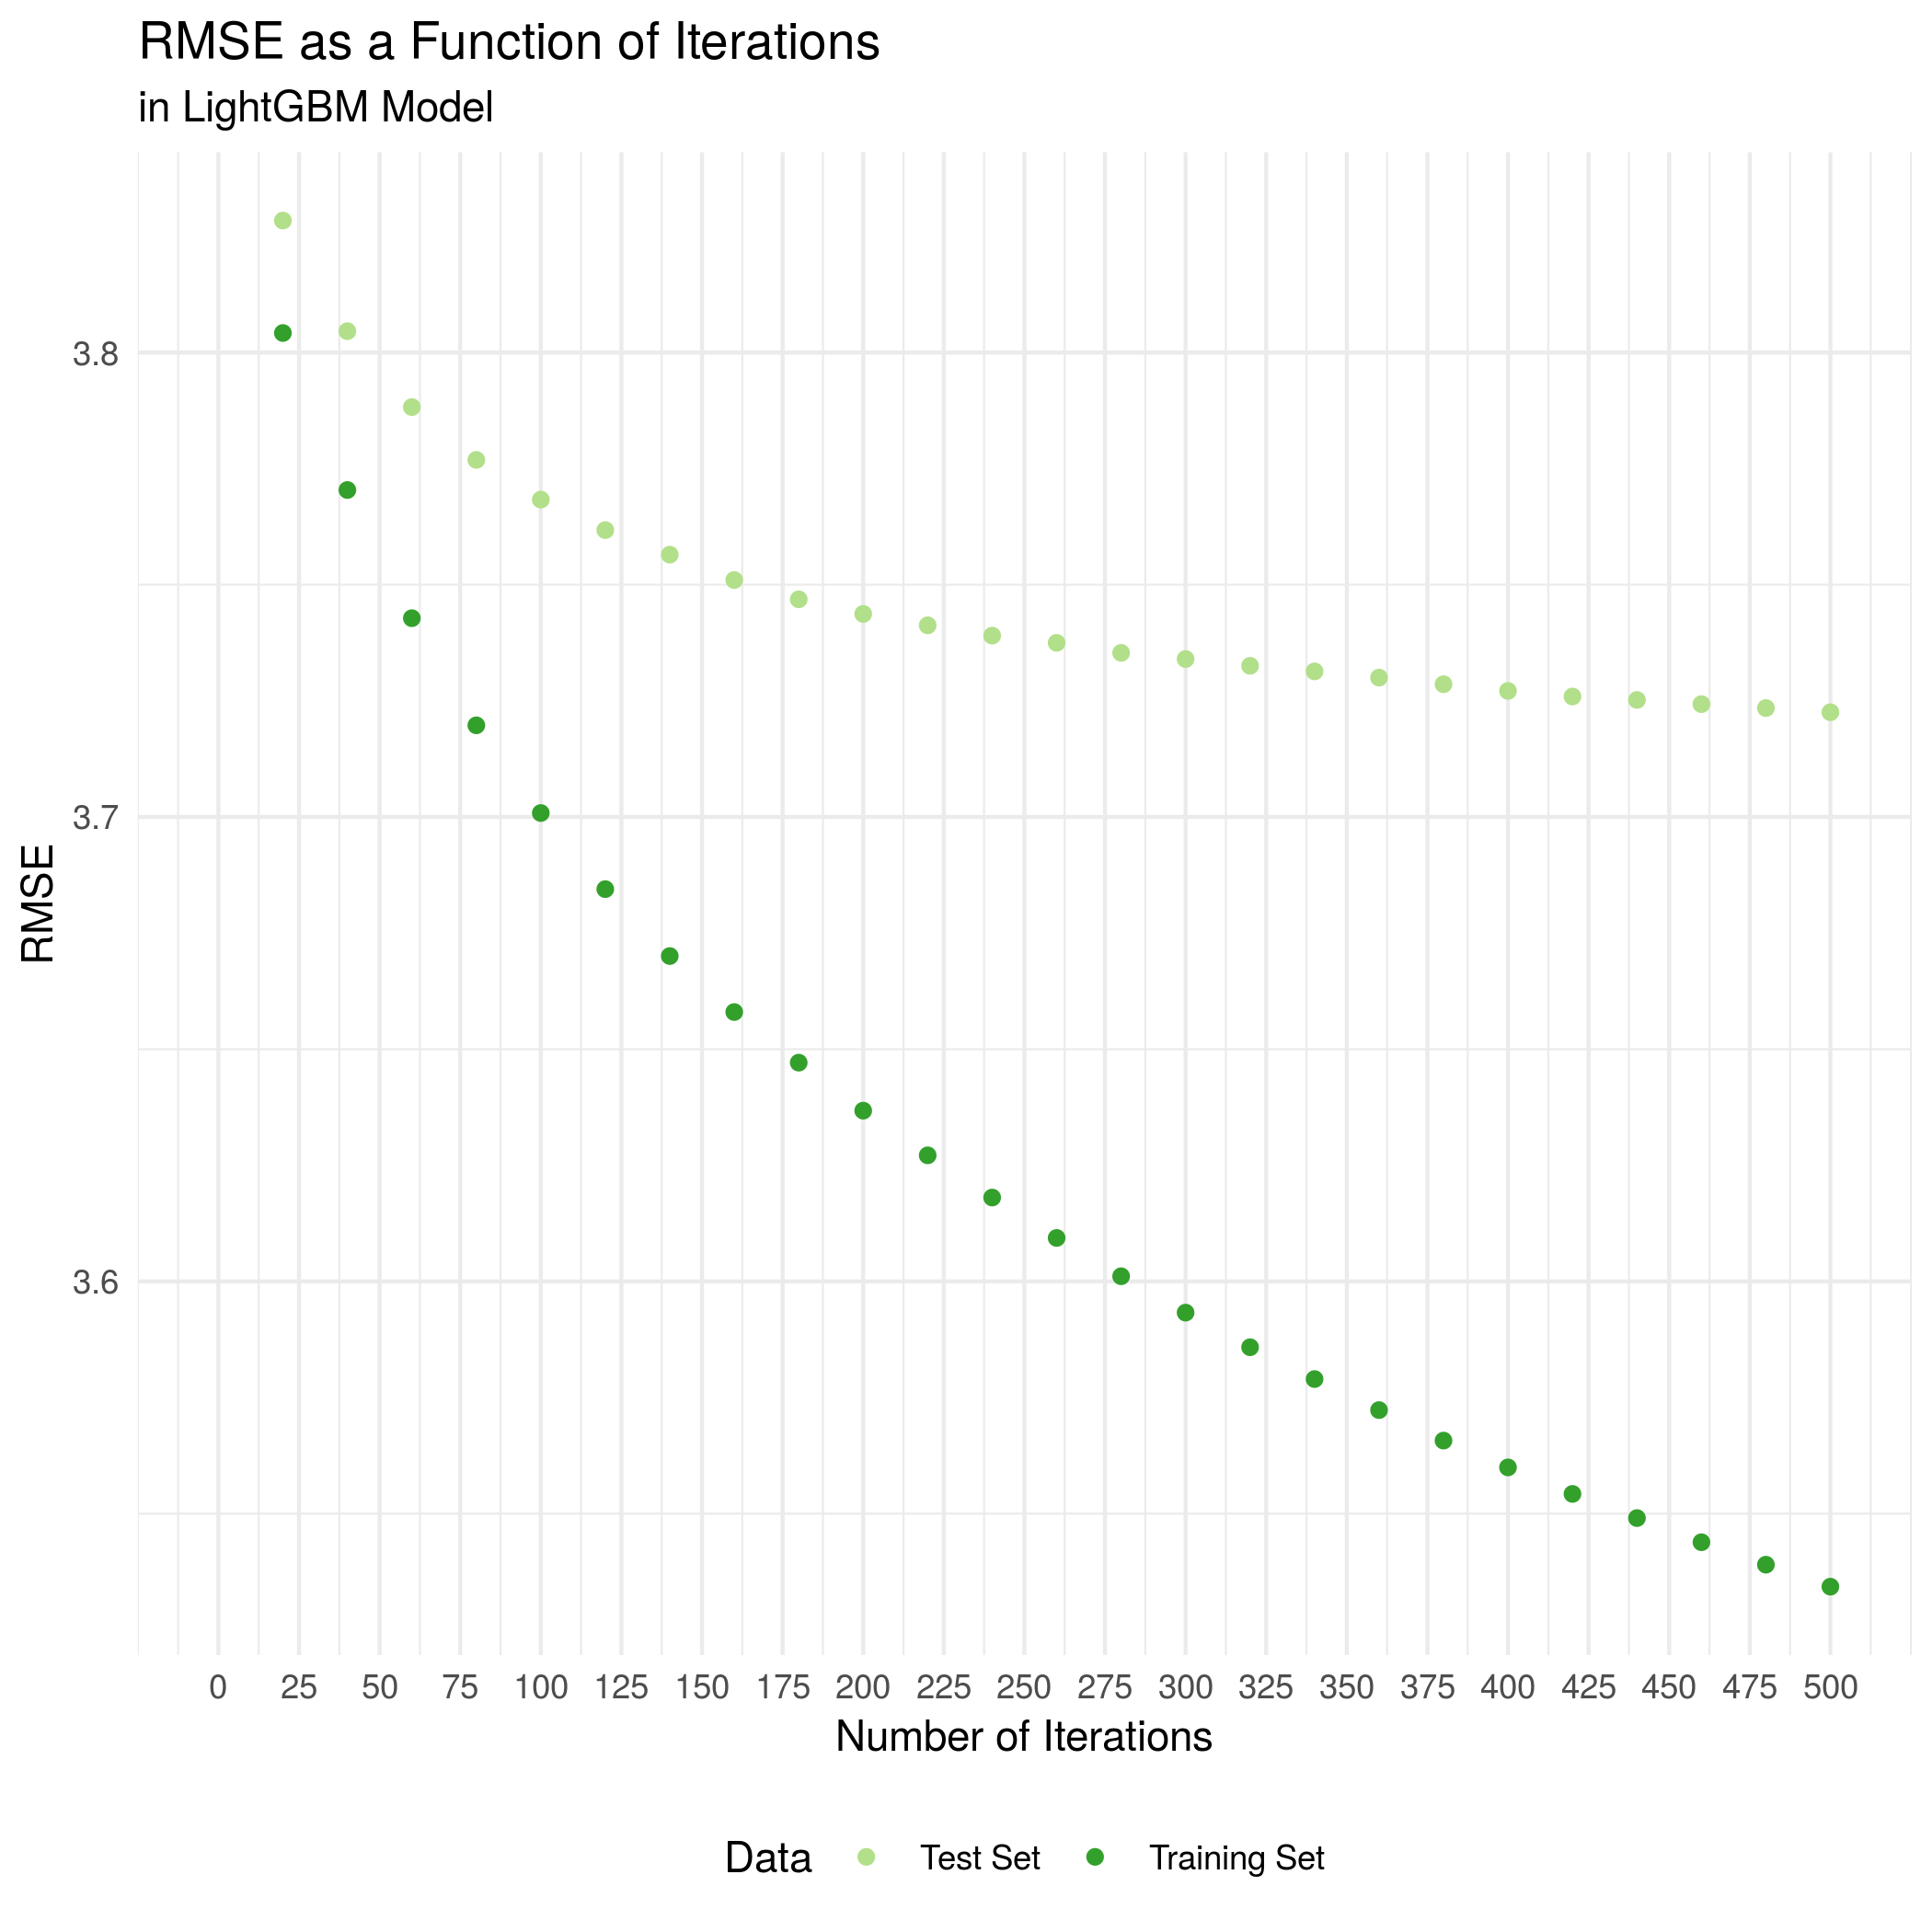
\includegraphics[height = 7cm, width = 7cm]{gbm_rmse_plot} \caption{RMSE as a function of iterations in LightGBM} \end{figure} As iterations increase, the training error becomes smaller and smaller, with decreasing change. The test set RMSE appears to become unchanging around $3.725$ after $350$ iterations. Note that the training and test error in this plot is found by subsetting the training data into two pieces for measuring errors. The real test metric is given in the table above, Now, the important features found by the algorithm is shown in Fig. 17. \begin{figure}[t] 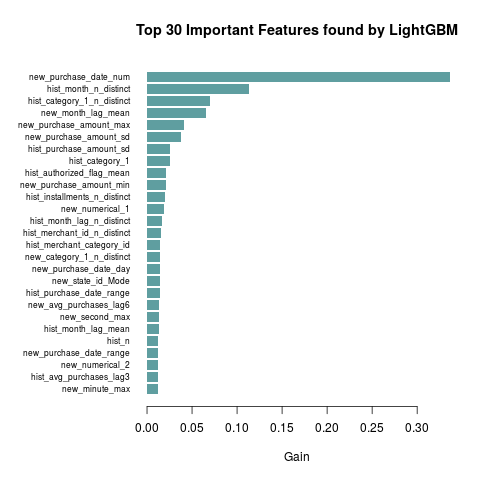
\includegraphics[scale = 0.4]{lgb_features_plot} \caption{Important features determined by the LightGBM algorithm} \end{figure} Most of the same features found important by the XGBoost model is found again by this model. The maximum purchase amount in new transactions is now dropped to fifth position whereas before it was second most important. The second most important feature now is number of distinct months of transactions in historic transactions.What is interesting to see now is that the number of historic transactions is at the bottom of the list, signifying that it is not as important as in the random forest or XGBoost models. Less than half the important features in this model are from historical transactions. Newer transaction features appear to be more relevant. 

\section{Conclusion}
Elo has given a big job to Kagglers, to predict loyalty scores for their card holders. Explanatory data analysis helped to find some insightful patterns in customer transactions such as when they shop and common merchants. Feature engineering helped to create new information from what was given from millions of transactional data. Numerous regression models were explored in this study to predict loyalty scores. It was found that the gradient boosted regression trees created the least error in predicting loyalty scores for Elo card holders. Furthermore, it was seen that this algorithm helped to determine which features are more important in determining scores. This can be helpful for Elo to look at when forecasting predictions for the future. In the future, it would be advised to look into how to remove noise from the features data, the ones originally given in the training and test data by Elo. The three features were not found in the top $30$ important features to explain loyalty scores. But Elo would not provide them if they weren't important. Thus further feature engineering or modeling techniques could be used to give these variables more predictability power. 

\section{Acknowledgment} 
I would first like to acknowledge Professor Vikas Ramachandra for his dedicated support in the machine learning for statistics course at Fordham University Gabelli School of Business Spring 2019. Despite teaching online, he was always available to answer questions. I would also like to acknowledge Louis Aslett for having Amazon Machine Images (AMIs) already set up with RStudio Server on them. Due to his publicly available AMIs, I could easily get a server running up on Amazon Web Services ready to do data manipulation, analysis and modeling. If you, the reader, would like to leverage the power of cloud computing for statistical analysis, please visit the following webpage: \href{http://www.louisaslett.com/RStudio_AMI/}{Louis Aslett's RStudio AMI}.  

\end{document}


